%%% Time-stamp: <mainrep.tex 19:57, 17 Jul 2016 by P Sunthar>
%%% $Log:$
% This document describes how to use iitbreport style
%********************************************************************

%\documentclass[11pt,a4paper,openright]{report}
\documentclass[oneside]{iitbreport}
\usepackage{graphicx}
\usepackage{multirow}
\usepackage{listings}
\usepackage{float}
\usepackage{amsmath,bm}
\usepackage{csvsimple}
\usepackage{hyperref}
\usepackage{longtable}

\newcommand{\specialcell}[2][c]{%
		\begin{tabular}[#1]{@{}c@{}}#2\end{tabular}}
	
\newcommand*{\captionsource}[2]{%
	\caption[{#1}]{%
		#1%
		\\\hspace{\linewidth}%
		\textbf{Source:} #2%
	}%
}

%\usepackage[pdfencoding=auto]{hyperref}
%%\selectlanguage{English}
%% Default spacing: 1.5
%% Default font size: 12pt
%% Default font: txfonts (similar to times new roman) 
%% Selectively comment out sections that you want to be left out but
%% maintaining the page numbers and other \ref
\includeonly{%
  intro/introduction,
  layout/layout,
  OpenFOAM/OpenFOAM,
  geometry/geometry,
  optimization/optimization,
  lit/literature,
  expt/experimental,
  Hoop_stress/Hoop_stress,
  surrogate_model_CFD/surrogate_model_CFD,
  surrogate_model_CFD_results/surrogate_model_CFD_results,
  rnd/results, 
  futureplan/futureplan,
  appendix,
  dec,abs,pub,ack
}

%%% Some commonly used packages (make sure your LaTeX installation
%%% contains these packages, if not ask your senior to help installing
%%% the packages)

\usepackage{booktabs}
\graphicspath{{expt/}}


%%% Macro definitions for Commonly used symbols
\newcommand{\Rey}{\ensuremath{\mathrm{Re}}}
\newcommand{\avg}[1]{\ensuremath{\overline{#1}}}
\newcommand{\tenpow}[1]{\ensuremath{\times 10^{#1}}}
\newcommand{\pder}[2]{\ensuremath{\frac{\partial#1}{\partial#2}}}

% Referencing macros
\newcommand{\Eqref}[1]{Equation~\eqref{#1}}
\newcommand{\Tabref}[1]{Table~\ref{#1}}
\newcommand{\Figref}[1]{Figure~\ref{#1}}
\newcommand{\Appref}[1]{Appendix~\ref{#1}}


\begin{document}
	
%%********************************Frontmatter***********************
% In frontmatter everything comes with roman numbering	
\pagenumbering{roman}
\setcounter{page}{1}

%*******************************************************************
%                         Title Page                            
%*******************************************************************
\title{Multi-Disciplinary Shape Optimization of Airship envelopes}
\author{Manideep Reddy Desham}

%% Print the date. Today's date comes by default, change it here to 
%% other date format, if required:

\date{\today}
%\date{03 Oct 2017}


%% The type of the report can be set here

\reporttype{AE 797 M.Tech. Project Report}
%\reporttype{A Thesis}
%\reporttype{A Dissertation}
%\reporttype{A Project Report}

%% Name of the degree
%\degree{Doctor of Philosophy}
%\degree{Master of Technology}


%% Department/Centre Name
\dept{Department of Aerospace Engineering}

%% Supervisor and cosupervisor/excosupervisor are not essential parts
%% of a report title page, as it is your report!

%% But if you **have** to put it uncomment these
\supervisor{Prof. Rajkumar S. Pant}
%\cosupervisor{Co-super name}
%\excosupervisor{External Supervisor}

%% Roll number
\rollnum{Roll No. 163010004}


\maketitle

%*******************************************************************
%                         Copyright Page                          
%******************************************************************* 
%\mycopyright                    

%*******************************************************************
%                         Dedication Page                         
%*******************************************************************
%\dedication[Dedicated to \ldots]        
%\addintoc{Dedication}

%*******************************************************************
%                        Certificate Page                         
%*******************************************************************
%\makecertificate[change title name]{report type} 
%\makecertificate{seminar report} 
%\makecertificate{thesis}
%\makecertificate{dissertation}
\makecertificate{project report}

%\addintoc{Certificate}

%*******************************************************************
%                         Approval Sheet                         
%*******************************************************************
%\makeapproval{thesis}
%\makeapproval{dissertation}

%*******************************************************************
%                          Declaration                           
%*******************************************************************
%%==================================dec.tex================================
%
\begin{Declaration}
\noindent
I declare that this written submission represents my ideas in my own words and where others' ideas or words have been included, I have adequately cited and referenced the original sources. I declare that I have properly and accurately acknowledged all sources used in the production of this report. I also declare that I have adhered to all principles of academic honesty and integrity and have not misrepresented or fabricated or falsified any idea/data/fact/source in my submission. I understand that any violation of the above will be a cause for disciplinary action by the Institute and can also evoke penal action from the sources which have thus not been properly cited or from whom proper permission has not been taken when needed.

%
%
%
%
%
%
%

\DecSign[ 03 Oct 2017]



%
\end{Declaration}
%========================================================================
















 
%\addintoc{Declaration}

%******************************************************************
%                          Abstract                             
%******************************************************************  
%============================= abs.tex================================
\begin{Abstract}
Stratospheric Airships are being considered as the aerial platform of choice for long endurance applications, especially for mounting next generation of communications payloads. Such airships are generally powered by solar propulsion systems, hence it is preferable for their envelopes to have flat upper surfaces for mounting solar panels.   

Most existing studies related to shape optimization of stratospheric airships assume their envelopes to be axisymmetric bodies of revolution, since the drag coefficient of such shapes can be estimated by 2D CFD analyses. But non-axisymmetric envelope shapes need 3D CFD analysis to be performed, which demands more computational effort. 

The present study aims at developing a surrogate based design optimization (SBDO) methodology for obtaining minimum drag shapes of stratospheric airship envelopes, which are non-body of revolution. A novel scheme for parameterization of envelope shapes of a given volume is presented, using modified Gertler Series 58 Shape Generator. Latin Hyper-cube Sampling is used to generate 100 shapes, and the volumetric drag coefficient (C DV ) of the envelope is determined at these points by carrying out 3-D CFD analysis using OpenFOAM\textsuperscript{\textregistered}. A simple Kriging surrogate model was fitted through these points, which predicted  \textbf{$ C _{DV} $  values within $ 2 \% $} accuracy at 15 uniformly distributed trial shapes. A shape corresponding to minimum C DV of this surrogate function was obtained using Genetic Algorithm optimizer, and was found to have a $ C _{DV} $ only slightly worse off than that of a reference GNVR shape, thus establishing the efficacy of this scheme.
\end{Abstract}
%=======================================================================
                    

%******************************************************************
%                         Contents list                         
%******************************************************************
%\figurespagefalse
%\tablespagefalse
\makecontents % Creats toc, lof, and lot

%******************************************************************
%                        Notations                              
%******************************************************************
\notations[4cm]{List of Symbols}      

%%********************************Mainmatter***********************
% In mainmatter everything comes with arabic numbering	
\cleardoublepage
\setcounter{page}{1}
\pagenumbering{arabic}

%******************************************************************
%                         Chapters                           
%****************************************************************** 

\newcommand{\etas}{\ensuremath{\eta_{\mathrm{s}}}}


\chapter{Background and Introduction}

\section{Stratospheric Airships}
In the present climate of growth in broadband-hungry telecommunication applications, wireless infrastructure providers are under continuous pressure to exploit the limited radio spectrum as efficiently as possible. In this context, high altitude platforms (HAPs) are increasingly being cited as having an important role to play in future systems and applications. They have the potential to exploit many of the best aspects of terrestrial and satellite based systems, while offering advantageous propagation characteristics. Such platforms may be airships or aircraft and for environmental considerations would ideally be solar powered.
\begin{figure}[htbp]
	\centering
	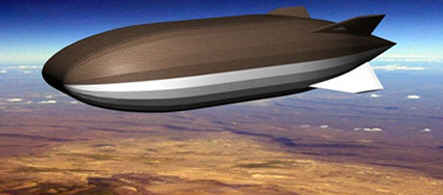
\includegraphics{intro/Stratellite.jpg}
	\caption{A stratospheric airship (Stratellite)}
	\label{Stratellite} %      only if needed 
\end{figure}

Keeping the above problem in mind, a stratospheric airship can be designed which can float at an altitude of 17-25 km and would be powered by direct solar energy extracted by photo-voltaic cells during day time and energy stored in the regenerative fuel cells during night time. The airship is required to stay aloft at a particular position despite of the wind gusts. So,the position should be corrected from time to time. This demands for the need of propellers using which the position of the airship at a particular altitude is corrected from time to time.

17-25 KM altitude is the place where little or no weather activities like rain, thunderstorms or cyclones takes place. At that altitude, things like pressure, density temperature and wind velocity remains constant or changes from season to season. So, this layer can be utilized to station our stratospheric airship.

 There are potentially many advantages of stratospheric airships compared to ground level telecommunication or satellite communication systems. Some of them are:
 
 \begin{itemize}
 	\item Larger ground coverage compared to ground level telecommunication systems like towers.
 	\item They can be used for strategic surveillance purposes by defence and military agencies.
 	\item They can be thought of an alternative to geostationary satellites with two potential advantages. One being low initial and operating costs involved. Second being the ability to update, repair and maintain the payload systems from time to time.
 	\item They can be used for communication purposes during emergency caused because of natural calamities or disasters since ground based telecommunication systems might not work properly at these times.
 \end{itemize}
 
\section{Motivation}

Unconventional non-axisymmetric shapes provides many advantages over conventional axisymmetric shapes for stratospheric airships because they can have flatter upper surface and is advantageous for capturing more solar irradiance. Existing literature has good amount of work on CFD analysis of axisymmetric shapes. But there is no considerable amount of analysis on non-axisymmetric shapes. The reason is obvious, 2D analysis can be easily done for axisymmetric shapes. But to do CFD analysis on non-axisymmetric shapes, we need to perform 3D CFD analysis. 3D analysis demands more computational effort which might not be available for many researchers.

There are many advantages for OpenFOAM\textsuperscript{\textregistered} like availability of source code, small size code (only 200 MB) and complete flexibility in usage. OpenFOAM\textsuperscript{\textregistered} also comes with an inbuilt meshing (\textit{Block mesh} and \textit{Snappy Hex Mesh}) and post-processing (\textit{Paraview}) utilities, both of which are known for their unique and advanced method of problem solving capabilities. \\

\section{Objective and Aims}
The project is divided into two stages namely Stage-1 and Stage-2. In Stage-1, existing CFD results available in the literature for four standard shapes will be reproduced by carrying out 3D CFD analysis using OpenFOAM\textsuperscript{\textregistered}. A methodology for carrying out multi-disciplinary optimization will be laid out. The methodology should be such that optimal shape of the envelope should be obtained in minimum amount of time and optimally utilizing computational resources. The objectives for Stage-2 are explained in Chapter \ref{future plan}

\section{Report layout}
\label{layout}

After providing a brief introduction to Stratospheric Airships outlining the aims and objectives of this study, Chapter \ref{literature} gives the detailed literature survey of various fields required for multi-disciplinary shape optimization. Chapter \ref{openfoam} gives a brief introduction about OpenFOAM. Section \ref{Advantages of openfoam} demonstrates the power, advantages and disadvantes of using OpenFOAM\textsuperscript{\textregistered}
Mesh generation using two utilities namely \textit{Gmsh} and \textit{SnappyHexMesh} are discussed in section \ref{mesh}. Section \ref{results} validates the OpenFOAM\textsuperscript{\textregistered} software with four axisymmetric standard shapes available in literature. Chapter \ref{geometry}  explains the modified gertler parameter technique used for the parameterization of geometry. This is also shown in Figure \ref{Report layout}.

Chapter \ref{optimization} gives a brief overview of need for a surrogate model in the optimisation routine and explains the concept of surrogate model, design of experiments and formulation of different surrogate models. Section \ref{test function} explains the surrogate based optimisation technique using a test function called Himmelblau function. It also validates the Genetic algorithm code by \cite{Xavier} which is used in subsequent chapters.

Chapter \ref{Surrogate model for CFD} gives the design space and design of experiment study parametres which will be used while building surrogate model in chaper \ref{Training data CFD}. Running the actual CFD simulations for building surrogate model of CFD is done in chapter \ref{Training data CFD}.  

Chapter \ref{Hoop stress} explains the concept of hoop stress and also gives the methodology to calucate it as given by \cite{alam2017thesis}. The results obtained while performing multi-disciplinary optimisation of aerodynamic drag combined with hoop stress are presented in chapter \ref{Final results}.
Figure \ref{Report layout} shows where different chapters of this report fit in the framework of Multi-disciplinary shape optimisation.

\begin{figure}[H]
	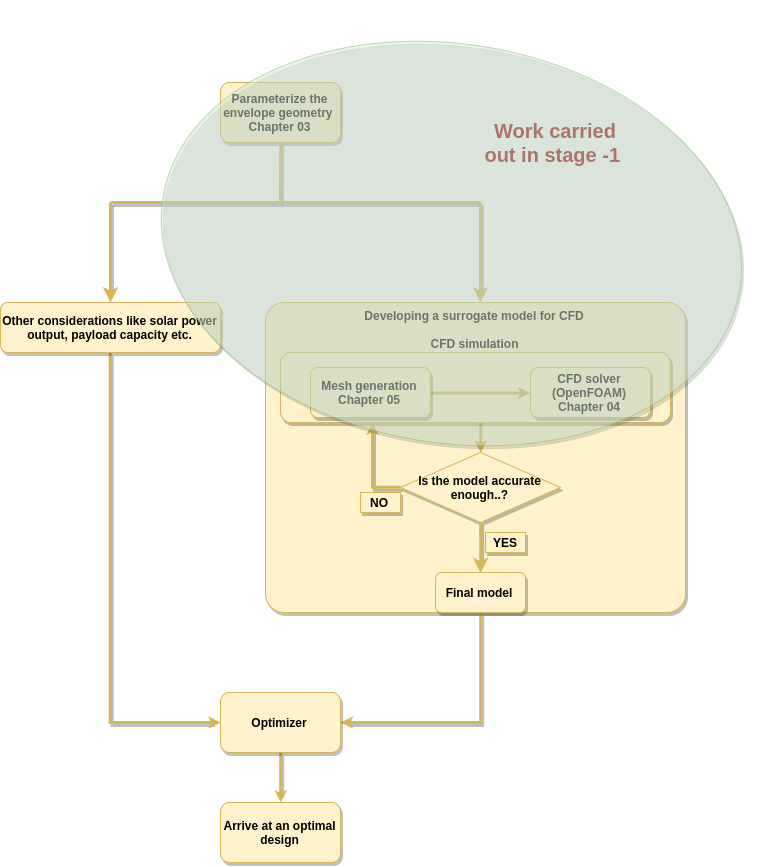
\includegraphics[width=\textwidth]{layout/layout.png} 
	\caption{Framework of multi-disciplinary shape optimization}
	\label{Report layout} %      only if needed 	
\end{figure}
%%
Next Chapter gives brief literature survey that has been carried out to understand the previous research carried out in the field of High Altitude Airships (HAA's) and shape optimisation.


%%% Local Variables: 
%%% mode: latex
%%% TeX-master: "../mainrep"
%%% End: 

%%


%%% Local Variables: 
%%% mode: latex
%%% TeX-master: "../mainrep"
%%% End: 

%\section{Report layout}

After providing a brief introduction to Stratoshperic Airships outlining the aims and objectives of this study, Chapter 2 ?????
 Chapter 3 gives the detailed literature survey of various fields required for multi-disciplinary shape optimization. Chapter 4  explains two of the many methods used for the parameterization of geometry. This is also shown in Figure \ref{Report layout}. Next, crisp introduction for advantages of using OpenFOAM\textsuperscript{\textregistered} is discussed in chapter 5. 

Mesh generation using two utilities namely Gmsh and \textit{SnappyHexMesh} are discussed in chapter 6. Collectively Chapters 3, 4 describe the work dork done in Stage-01. A brief introduction of methodology for optimization is given in chapter 07. However optimization will be done in stage -02 along with other considerations as shown in \ref{Report layout}. 

Finally chapter 8 discusses the results obtained while validating the results present in literature for various standard airship shapes using OpenFOAM\textsuperscript{\textregistered}. Finally chapter 8 gives the future work that will be performed in stage -02. The workflow for the total project is shown in Figure \ref{Report layout}. The blocks present in transparent oval is the work completed in stage 1. 

\begin{figure}[htbp]
	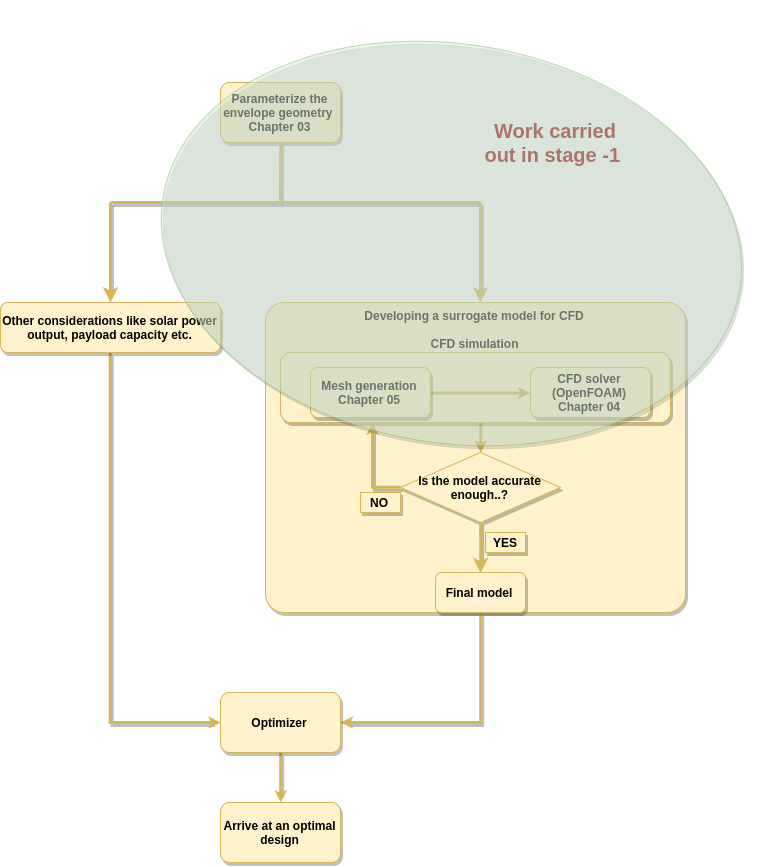
\includegraphics[width=\textwidth]{layout/layout.png} 
	\caption{Work flow of multi-disciplinary shape optimization}
	\label{Report layout} %      only if needed 	
\end{figure}
%%


%%% Local Variables: 
%%% mode: latex
%%% TeX-master: "../mainrep"
%%% End: 


\chapter{Literature Survey}
\label{literature}
This chapter presents the research carried out by different individuals in the field of shape optimisation.

Ghani[\citenum{OsamaAbdulGhani2013}] used Non Uniform Rational B-Splines (NURBS) for envelope geometry parameterization of passenger car and constructed a response surface model on the geometries to obtain drag coefficients. Finally, the design exploration was performed using the response surface model instead of actual CFD simulations.

Alam[\citenum{alam2016mdo}] selected \textit{Gertler Series-58} $ \; $ [\citenum{gertler1950}] shape generation for optimization studies, in which the envelope shape is driven by four shape parameters and fineness ratio. Wang et al.[\citenum{Wang2010}] proposed a geometry parameterization algorithm for axisymmetric bodies using four shape parameters namely \textit{a,b,c,d} and length \textit{l}.

Kanikdale et al.[\citenum{kanikdale2004multi}] has taken GNVR shape [\citenum{gnvr2000}]  as baseline reference and validated their ANSYS\textsuperscript{\textregistered} \textit{Fluent} results with it. Geometry has been parameterized using six design parameters and response surface based on CFD results was fitted. With low fidelity analysis using the formula by Gillett et al.[\citenum{cheeseman1999}]. An improvement of 1.3 \% was observed in $ C_{DV} $. Whereas using CFD analysis, they found that the drag for optimized shape is 27 \% greater than GNVR hull shape. By this, they concluded that the formula given by Gillet and Khoury cannot be used for optimization purpose.

Kale et al.[\citenum{Kale2005a}] proposed a generic methodology for determination of drag coefficient of an aerostat envelope using CFD. The envelope was parameterized in terms of six geometric coefficients, and a shape generation algorithm was developed. They have studied around 600 feasible shaped using ANSYS\textsuperscript{\textregistered} \textit{Fluent} CFD package and fitted a quadratic response surface using Design-Expert package. They taken a composite objective function involving aerodynamic drag, structural stress and surface area (so weight) of the envelope. They have observed that the location of maximum thickness affects the drag mostly. 

Ram et al.[\citenum{Ram2010}] parameterized the shape using the formulation proposed by Kanikdale et al.[\citenum{kanikdale2004multi}] and arrived at optimum shape using hybrid Genetic Algorithm (GA). The objective function was to maximize its payload while incorporating considerations of aerodynamics, structures and flight mechanics.

Wang et al.[\citenum{Wang2010}] have tested a scaled down model of Zhiyuan - 1 airship in a 3.2 m diameter wind tunnel and installed roughness strips on the surface of hull to trip the flow from laminar to turbulent. They studied the effect of lengthwise location of these strip on the its aerodynamic characteristics at different angles of attack and side slip. They have reported large sets of experimental data for bare hull, hull with fins and hull with fins, gondola. They concluded  that the drag almost doubled because of change of flow condition from laminar to turbulent.

Suman et al.[\citenum{Suman2011}] tried to reproduce the experimental results of Wang et al.[\citenum{Wang2010}] using computational fluid dynamics. To simulate the turbulence strips installed by  Wang et al.[\citenum{Wang2010}] on the surface of the hull, Suman et al.[\citenum{Suman2011}] modeled transition location in CFD which changes the flow from laminar to turbulent. It has been observed that although Wang et al.[\citenum{Wang2010}] provided strips at the leading edge, the flow has not been tripped to turbulent because of favorable pressure gradient.

Comprehensive results for the effect on size and payload capability of airship of various factors like, altitude, latitude, pressure difference, helium purity etc. has been published by Chen et al.[\citenum{Chen2010}]. The calculation is carried out for NPL shape.


Liu et al.[\citenum{Liu2013c}] carried out numerical calculations about the test model to investigate the aerodynamics behaviour. They confirmed the lower drag behaviour of \textit{Zhiyuan-1} airship. They discussed the influence of gondola and fins on the pressure distribution.

Ceruti et al.[\citenum{Ceruti2013b}] defined a shape which is non body of revolution using five design parameters. They have found the drag coefficient for 10 such combinations of design parameters and used interpolation based approach for estimation of drag coefficient of any given shape. They used different optimization techniques to arrive at a configuration of minimum drag and weight. 


\section{Recent work in the field}

A brief summary of recent work done by Alam [\citenum{alam2017thesis}] in the field of multi-disciplinary shape optimization is given below. 

\textbf{Surrogate model for CFD analysis:}
For CFD analysis, 60 simulations have been carried out and fitted into the \textit{Kriging} surrogate model toolbox developed by Viana et al.[\citenum{viana2014metamodeling}]. This has been coupled with the optimizer without having the need to do CFD routine every time.

\textbf{Shape generation algorithm:}
The shape generation algorithm proposed by Gertler[\citenum{gertler1950}] called \textit{Gertler Series 58 Shape Generator} has been used instead of that by Wang et al.[\citenum{Wang2010}]. Efficacy of this shape generator has been demonstrated by capturing different standard airship shapes. 

\textbf{Sizing and Optimization:} 
A new sizing methodology has been developed by Alam et al.[\citenum{alam2014mdo}] and optimization has been carried out using MATLAB Global optimization Toolbox and SIMANN optimizer.

The next Chapter investigates envelope shape generation algorithms for non-axisymmetric shapes because the existing literature has only algorithms for axisymmetric shapes. 





%%% Local Variables: 
%%% mode: latex
%%% TeX-master: "../mainrep"
%%% End: 

\chapter{Introduction to OpenFOAM\textsuperscript{\textregistered}}

\label{openfoam}

OpenFOAM\textsuperscript{\textregistered} is a Free Open Source Software (FOSS) where we can get the source code along with binary executable for all the solvers. The FOAM project (precursor to OpenFOAM\textsuperscript{\textregistered}) was created at Imperial College London in the late 80s and early 90s by Henry Weller, along with Hrvoje Jasak, using the new object-oriented programming language C++. Succeeding the commercial software FOAM, OpenFOAM\textsuperscript{\textregistered} was released in 2004 as free and open-source software under the GNU General Public License (GPL), a widely used free software license, which guarantees end users the freedom to run, study, share and modify the software.

OpenFOAM\textsuperscript{\textregistered} has been used instead of ANSYS\textsuperscript{\textregistered} \textit{Fluent} because it has many potential advantages. Here we can modify the existing solvers/models to suit our particular needs, compile them and add them to our library. One distinguishing feature of OpenFOAM\textsuperscript{\textregistered} is its syntax for tensor operations and partial differential equations (PDEs) that closely resembles the equations being solved. For example, the equation: 
\begin{equation}
\dfrac{\partial(\rho U)}{\partial t} + \nabla \boldsymbol{\cdot} \phi U - \nabla \boldsymbol{\cdot} \mu \nabla U = - \nabla p
\end{equation}
is represented by the code: 
\begin{verbatim}
Solve
(
	fvm :: ddt(rho,U)
	+ fvm :: div(phi,U)
	- fvm :: laplacian(mu,U)
	==
	-fvc :: grad(p)
);

\end{verbatim}

Thus we can see that all the mathematical operators like divergence, curl, gradient, laplacian etc. are well defined in OpenFOAM\textsuperscript{\textregistered}. OpenFOAM\textsuperscript{\textregistered} treats fluid, structural, thermal or acoustic or any other field problems in the exactly same way as long as there are governing equations in them and they can be written in conservative form. It uses finite volume discretization method. Whenever we are programming any new solver, 90 percent of the code remains same with baseline solver and changes to be made are less than 10 percent. Thus using OpenFOAM\textsuperscript{\textregistered}, There is no need to write the entire code right from scratch every time. We can just edit the existing solver and save lot of time.

Automatic mesh generation utility called \textit{SnappyHexMesh} comes along with OpenFOAM where in we have to give .stl or .obj file of geometry and specify the level of refinement needed. The rest is taken care by it. This is particularly useful when we have to couple CFD analysis to the optimizer. \textit{SnappyHexMesh} is still in development phase and is getting better with every release.

The absence of Graphical User Interface (GUI) can be taken as an advantage because we come to know the actual physics of flow happening behind the scene. If you become moderately expert in OpenFOAM\textsuperscript{\textregistered} then it saves a lot of time because we can programatically control all the inputs/outputs and we can automate many processes right from mesh generation to post processing.

OpenFOAM\textsuperscript{\textregistered} comes with a Open Source CFD post processing utility known as \textit{ParaView}.\textit{ParaView} accepts both point field data as well as volume field data. Since we solve Navier Stokes equations using Finite Volume Approach, at the end we are provided with data at the centre of cells. In this case, \textit{ParaView} is very useful. On the other hand, \textit{Tecplot\textsuperscript{\textregistered}} (commercially available CFD post software) accepts data only at the vertices.

\section{OpenFOAM\textsuperscript{\textregistered} for CFD researchers}

The main difficulty for engineers in using OpenFOAM\textsuperscript{\textregistered} is that it is not user friendly. Learning curve for openFOAM\textsuperscript{\textregistered} is very steep. But learning it adds value to one's skill set. OpenFOAM\textsuperscript{\textregistered} is used in the cases where ANSYS\textsuperscript{\textregistered} \textit{Fluent} fails. Because it has the transparency within it. It is arguably equally powerful as ANSYS\textsuperscript{\textregistered} \textit{Fluent}. To do any simulation using OpenFOAM\textsuperscript{\textregistered}, We have to basically think all the way back from vector Calculus to advanced topological errors. This will not only make us think like a computational scientist but will create awareness about how do we go about solving a problem from its inception to execution.



 

There are also many graphical user interfaces available for OpenFOAM\textsuperscript{\textregistered}. However using gui, we can do only limited tasks. OpenFOAM\textsuperscript{\textregistered} also comes with many utilities using which we can convert mesh generated by third party meshing tools like ANSYS\textsuperscript{\textregistered} \textit{Gambit}, \textit{Gmsh}, etc to OpenFOAM\textsuperscript{\textregistered} format.

OpenFOAM\textsuperscript{\textregistered} also comes with parallel processing utilities using which we can decompose, reconstruct and redistribute the computational case to perform parallel calculations, at times better than other CFD software. All these things makes OpenFOAM\textsuperscript{\textregistered} suitable for general engineers because we come to know whats happening behind the screen rather than just clicking the buttons. 


\section{Computational mesh generation using \textit{SnappyHexMesh}}

\textit{SnappyHexMesh} is a hexahedral unstructured mesh generation tool included in the distribution of OpenFOAM\textsuperscript{\textregistered}. \textit{SnappyHexMesh} can use a 3-D .stl surface and iteratively build a mesh upon it. Some options allow construction of several cell layers of a controllable height above the 3D surface.This feature makes it possible to have a refined mesh in the region of high velocity gradients, close to the surface.  Near the surface, the mesh is refined and cells are splitted acoordingly. The process is explained in Figure ~\ref{Snappy Hex Mesh} .Several regions can be selected to be refined to a desired level, and this method creates mesh of a cell aspect ratio close to 1.This is done in order to ensure that OpenFOAM\textsuperscript{\textregistered} can solve the numerical problems with the highest efficiency and accuracy using meshes generated with \textit{SnappyHexMesh}. The meshing tool \textit{SnappyHexMesh} can be run in parallel on a computer cluster or a PC.

\begin{figure}[htbp]
	\centering
	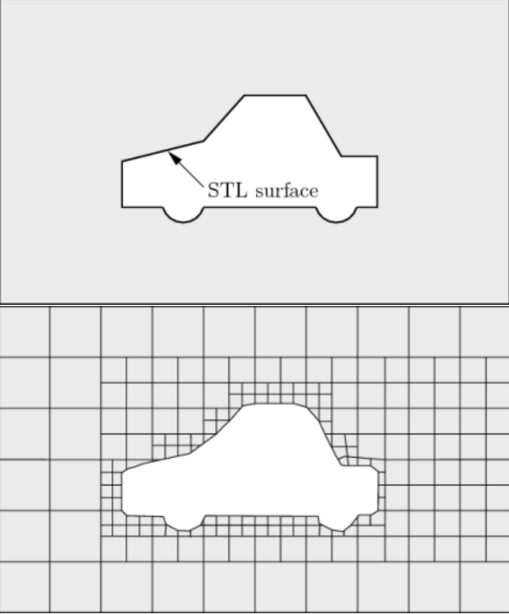
\includegraphics[width=200 pt]{mesh/snappyHexMesh.png}
	\caption{Surface snapping process in \textit{snappyHexMesh} }
	\label{Snappy Hex Mesh} %      only if needed
\end{figure} 

Although in the Figure ~\ref{Snappy Hex Mesh}, it is shown for 2D, \textit{SnappyHexMesh} is a 3D meshing utility.

\section{Validation of OpenFOAM\textsuperscript{\textregistered} CFD results}
\label{results}

This section describes the values of $C_{DV}$ obtained for four standard axisymmetric LTA envelope shapes, viz., GNVR \cite{Ram}, NPL \cite{cheeseman2012} Zhiyuan-1 \cite{zhiyuan}, and Wang \cite{Wangshape}, using OpenFOAM\textsuperscript{\textregistered}, and a comparison with the quoted values. 
Fig. \ref{All profiles} shows these four profiles. All the simulations were carried at zero degree angle of attack.

\begin{figure}[H]
	\centering
	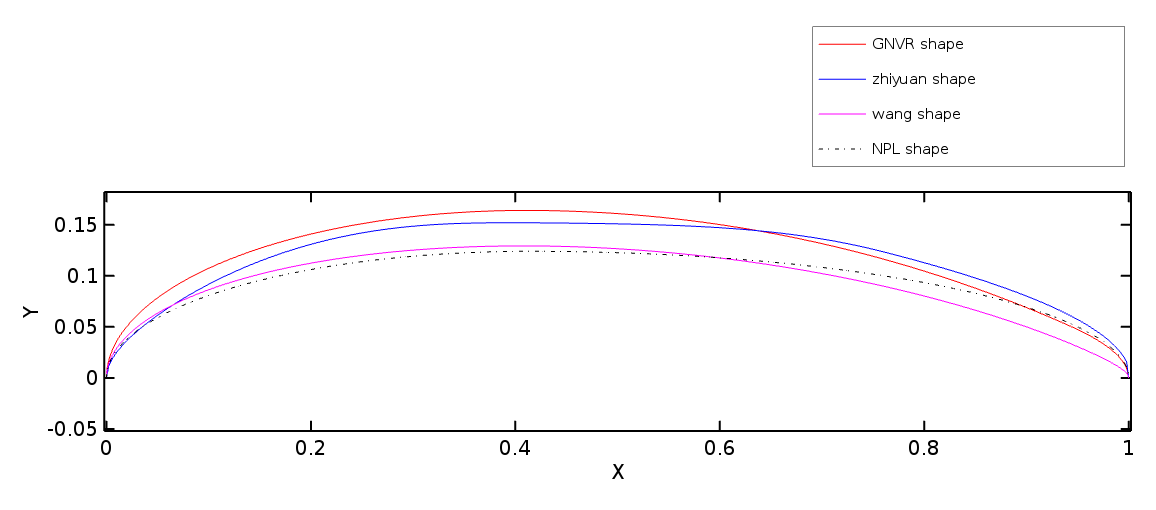
\includegraphics[width=400 pt]{rnd/all_profiles.png}
	\caption{Four standard shapes available in literature}
	\label{All profiles} 
\end{figure}
The specifications of machine, operating system, and software used in this study are as follows:
\begin{itemize}
	\item Model name = Intel(R) Xeon(R) CPU E5-2650
	\item Number of physical cores = 40
	\item Processor speed = 2.8 GHz
	\item Operating system = Cent OS 7.4
	\item OpenFOAM\textsuperscript{\textregistered} version = 4.1
\end{itemize}
Following subsections shows flow conditions, solver parametres and results of CFD simulation carried on the above mentioned standard shapes. 

\subsection{GNVR shape \cite{Ram}}
The GNVR shape \cite{Ram} is named after late Prof. G.N.V Rao of Indian Institute of Science, Bengaluru. It consists of three standard geometrical constructs, viz, ellipse, circle and parabola. The entire envelope shape is parametrized in terms of its maximum diameter ($D$), as follows:
\begin{center}
	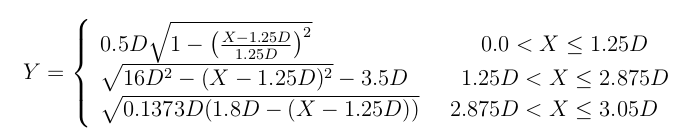
\includegraphics[width= 200 pt]{rnd/GNVR_equations.png}
\end{center}
Fig. \ref{prismlayers} shows the mesh near the surface of GNVR shape to resolve the boundary layer.
\begin{figure}[H]
	\centering
	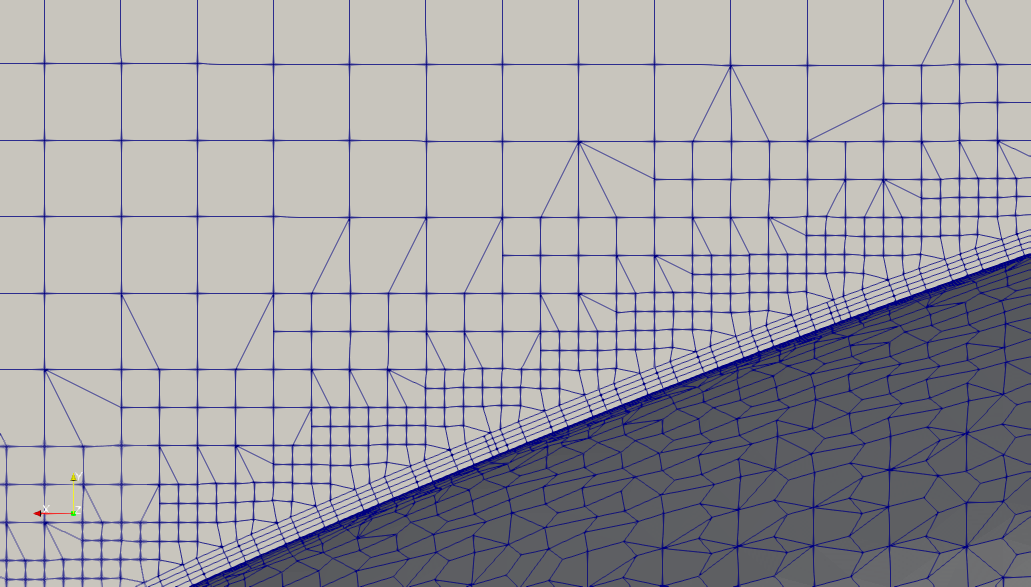
\includegraphics[width=300 pt]{rnd/prism_layer.png}
	\caption{Prism layers on the surface of GNVR to capture boundary layer}
	\label{prismlayers} %      only if needed
\end{figure}


The flow conditions used for the simulation are similar to that of Kanikdale et al. \cite{Kanikdale}. Taking advantage of the axisymmetric nature of GNVR shape, its 3D CFD analysis was carried out only for 1/4 of its shape. The flow conditions and solver parameters are shown in Table \ref{Flow conditions and solver parametres for GNVR shape}

\begin{table}[H]
	\caption{Flow conditions and solver parametres for GNVR shape}
	\label{Flow conditions and solver parametres for GNVR shape}
	\centering
	\begin{tabular}{ll}
		\hline \hline
		Flow Conditions & Solver parametres  \\ \hline \hline
		
		$ Velocity = 50.339 \; m/s$ & $Number \; of \; cells = 646,639$    \\  
		$ Pressure = 101325 \; Pa $ & $ Number \; of \; parallel \; cores = 20 $     \\
		$ Density = 1.225 \; kg/m^{3} $ & $ Time \; taken \; for \; solution = 475~s  $    \\
		$ Reynolds \; number = 34.783 * 10^{6} $ &    \\
		$ Turbulence \; model = k - \epsilon $ &     \\
		\hline
	\end{tabular}
	%	\end{ruledtabular}
\end{table}





The variation of Pressure coefficient ($C_{P}$) along the envelope length obtained using OpenFOAM\textsuperscript{\textregistered} is compared with that of using ANSYS\textsuperscript{\textregistered} \textit{Fluent} by Kanikdale et al. \cite{Kanikdale} and Panel method by Narayana and Srilatha \cite{srilata}. 

\begin{figure}[H]
	\centering
	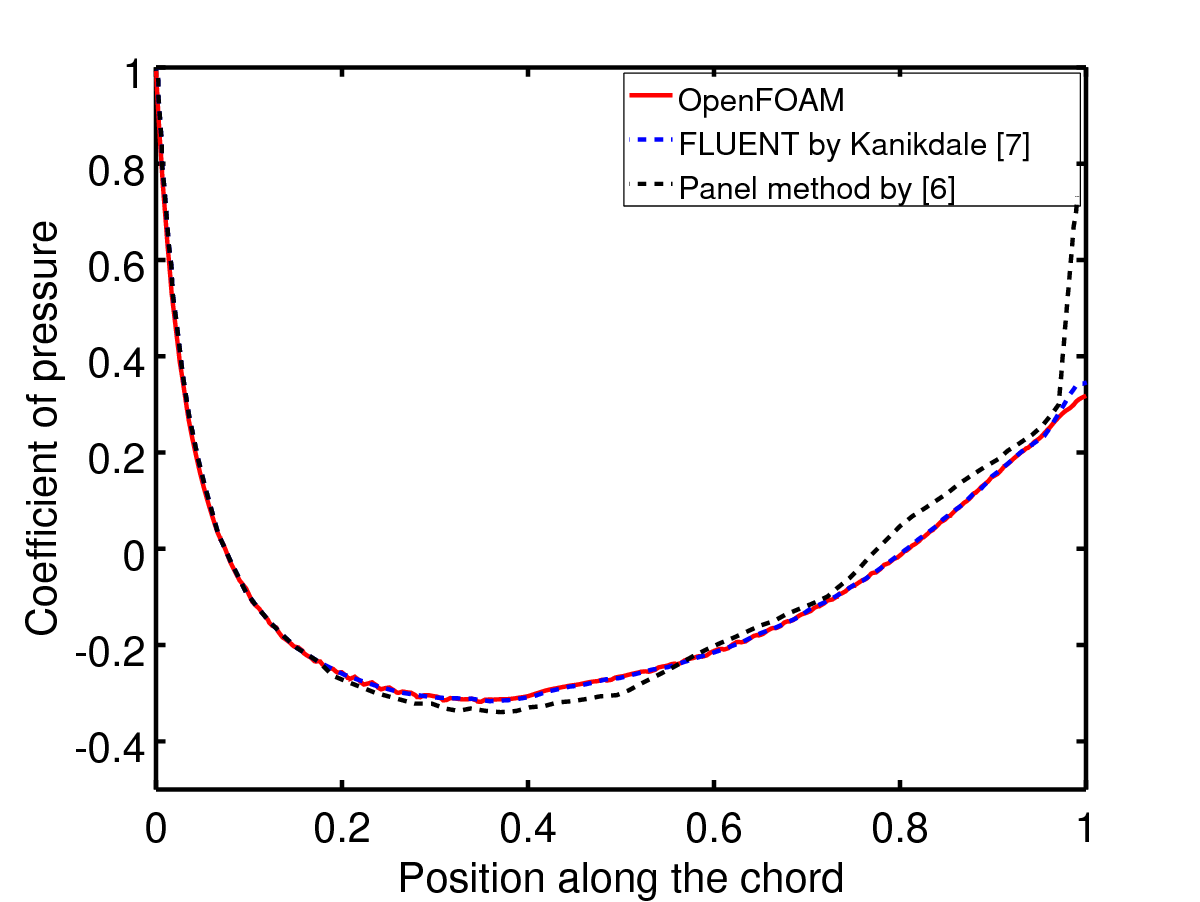
\includegraphics[width=270 pt]{rnd/GNVR_cp.png}
	\caption{$C_{P}$ distribution for GNVR profile obtained by OpenFOAM\textsuperscript{\textregistered}, Source Panel Method \cite{srilata} and ANSYS\textsuperscript{\textregistered} \textit{Fluent} \cite{Kanikdale}}
	\label{fig:GNVR pressure distribution} %      only if needed
\end{figure}

It can be observed from Fig. \ref{fig:GNVR pressure distribution} that the $C_{P}$ distribution obtained by OpenFOAM\textsuperscript{\textregistered} matches well with that obtained by ANSYS\textsuperscript{\textregistered} by Kanikdale et al. \cite{Kanikdale} along the entire envelope length, except at the trailing edge, where the flow is separated. The distribution obtained by Panel Method \cite{srilata} shows very high pressure recovery at trailing edge because attached flow is assumed, and the \textit{Kutta} condition is satisfied.

\subsection{Zhiyuan-1 shape \cite{zhiyuan}}

The equation that define the Zhiyuan-1 shape is:
\begin{center}
	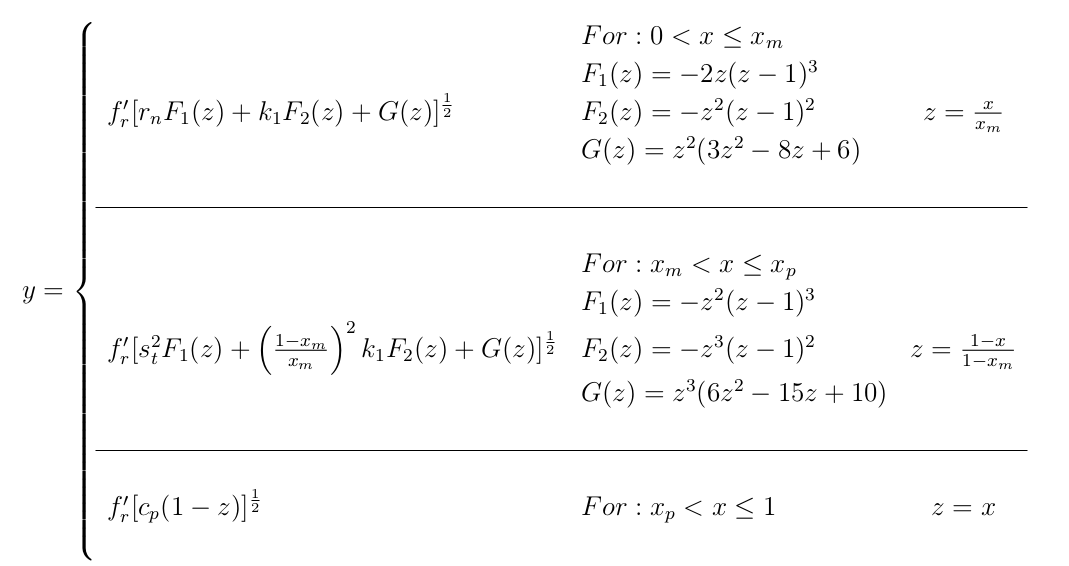
\includegraphics[width= 400 pt]{rnd/zhiyuan_equations.png}
\end{center}
Values of the constants mentioned above are as follows:

$ x_{m} = 0.393591, \quad x_{p} = 0.7570323,\quad r_{n} = 0.5070992,\quad k_{1} = 0.291256,\quad c_{p} = 2.735107,\quad f_{r}^{'} = 0.1515518 \quad and \quad  s_{t} = 3.236105 $


Suman et al. \cite{suman} carried out a Reynolds-Averaged Navier - Stokes (RANS) simulation to reproduce the results obtained by Wang et al. \cite{zhiyuan} for transition assumed at the leading edge itself, i.e., for a fully turbulent flow. They have also obtained results for various assumed locations of the transition points, resulting in pockets of laminar and turbulent regions in the computational domain.\\
In the present study, a 3-D CFD analysis for Zhiyuan-1 shape was carried out and pressure distribution is shown in Fig. \ref {fig:Zhiyuan-1 pressure}. 
\begin{figure}[H]
	\centering
	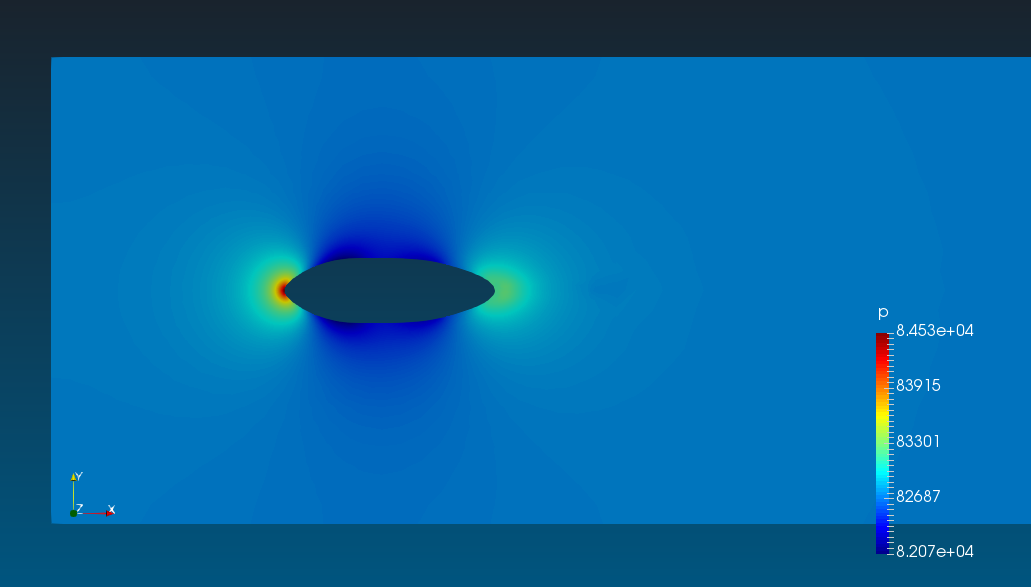
\includegraphics[width=300 pt]{rnd/pressure_zhiyuan.png}
	\caption{Pressure distribution on Zhiyuan-1 airship shape}
	\label{fig:Zhiyuan-1 pressure} %      only if needed
\end{figure}

The results were obtained only for one half of the envelope and `SymmetryPlane' boundary condition was incorporated for the other half to reduce the computational time.

The flow conditions used for the simulation were same as used by Suman et al. \cite{suman} and Wang et al. \cite{zhiyuan} and is given in Table \ref{Flow conditions and solver parametres for Zhiyuan-1 shape}

\begin{table}[H]
	\caption{Flow conditions and solver parametres for Zhiyuan-1 shape}
	\label{Flow conditions and solver parametres for Zhiyuan-1 shape}
	\centering
	\begin{tabular}{ll}
		\hline \hline
		Flow Conditions & Solver parametres  \\ \hline \hline
		
		$ Velocity = 60.39 \; m/s$ & $Number \; of \; cells = 2,982,639$    \\  
		$ Pressure = 101325 \; Pa $ & $ Number \; of \; parallel \; cores = 8 $     \\
		$ Density = 1.225 \; kg/m^{3} $ & $ Time \; taken \; for \; solution = 4534 \; s  $    \\
		$ Reynolds \; number = 2.4 * 10^{6} $ &    \\
		$ Turbulence \; model = \kappa \omega \; SST $ &     \\
		\hline
	\end{tabular}
	%	\end{ruledtabular}
\end{table}


Fig. \ref{Zhiyuan_OF_RANS} shows a comparison between the $C_{P}$ distribution for Zhiyuan-1 envelope shape using  OpenFOAM\textsuperscript{\textregistered} with ANSYS\textsuperscript{\textregistered} \textit{Fluent} and experimental results quoted by Wang et al. \cite{zhiyuan}
\begin{figure}[H]
	\centering
	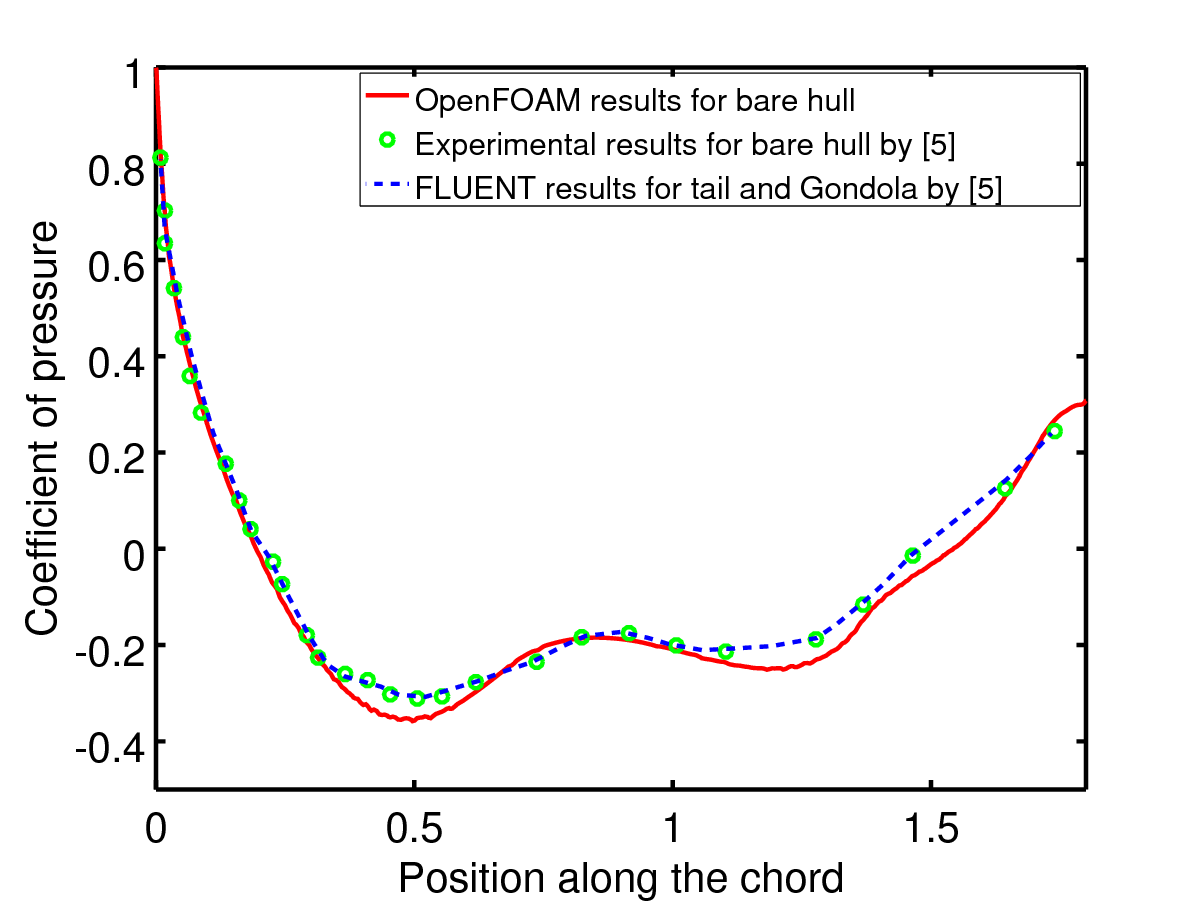
\includegraphics[width=270 pt]{rnd/zhiyuan_cp.png}
	\caption{$C_{P}$ distribution for Zhiyuan-1 shape using OpenFOAM\textsuperscript{\textregistered}, Experiments \cite{zhiyuan} and ANSYS\textsuperscript{\textregistered} \textit{Fluent} \cite{zhiyuan}}
	\label{Zhiyuan_OF_RANS} %      only if needed
\end{figure}

Table \ref{Zhiyuan -1 Cdv} compares the components of $C_{DV}$ obtained using OpenFOAM\textsuperscript{\textregistered} and RANS \cite{suman}.

\begin{table}[H]
	\centering
	\caption{\label{Zhiyuan -1 Cdv} Comparison of OpenFOAM\textsuperscript{\textregistered} results with RANS \cite{suman} for Zhiyuan -1 shape}
	%\begin{ruledtabular}
	\begin{tabular}{cccc}
		\hline \hline
		& OpenFOAM\textsuperscript{\textregistered} & RANS \cite{suman} & \% error    \\ \hline \hline
		
		$ C_{DV} (Viscous)$ & 0.01989 & 0.01890 & 5.3    \\  
		$ C_{DV} (Pressure) $ & 0.00583 & 0.00568 & 2.8    \\
		$ C_{DV} (Total) $ & 0.02573 & 0.02456 & 4.8    \\  \hline
	\end{tabular}
	%	\end{ruledtabular}
\end{table}


\subsection{Wang Shape \cite{Wangshape}}
Wang et al. \cite{Wangshape} proposed a new shape exploring the better shapes in the view of multi-disciplinary optimization. The geometry is defined by five shape parameters namely \textit{a, b, c, d} and length \textit{l}. The original equation proposed by Wang et al.\cite{Wangshape} is given by Eq. \ref{wang_eqn}:
\begin{equation}
64(y^{2} + z^{2}) = a(l-x)\left( bx - l \sqrt{c} + \sqrt{c l^{2} - dlx} \; \right) 
\label{wang_eqn}
\end{equation}

The values taken for the parameters of Wang shape are as follows: \\
\quad \textit{a = 7.447  \quad b = 2.072  \quad  c = 9.010 \quad d = 7.981} \quad and \quad \textit{l = 194.0} \\

For the sake of convenience, geometry is scaled down by length (\textit{l}) in all directions.
Wang shape defined by Eq. \ref{wang_eqn} is a body of revolution and also can be obtained by rotating the profile given by Eq. \ref{wang_eqn_2} through $ 360^{o} $.
\begin{equation}
y = \dfrac{\sqrt{a(l-x)\left( bx - l \sqrt{c} + \sqrt{c l^{2} - dlx} \; \right)}}{8} 
\label{wang_eqn_2}
\end{equation}

The flow conditions and solver parameters used for the simulation are shown in Table \ref{Flow conditions and solver parametres for Wang shape}:

\begin{table}[H]
	\caption{Flow conditions and solver parametres for Wang shape}
	\label{Flow conditions and solver parametres for Wang shape}
	\centering
	\begin{tabular}{ll}
		\hline \hline
		Flow Conditions & Solver parametres  \\ \hline \hline
		
		$ Velocity = 51 \; m/s$ & $Number \; of \; cells = 1,060,202$    \\  
		$ Pressure = 8750 \; Pa $ & $ Number \; of \; parallel \; cores = 8 $     \\
		$ Density = 1.225 \; kg/m^{3} $ & $ Time \; taken \; for \; solution = 2865 \; s  $    \\
		$ Reynolds \; number = 3.01 * 10^{6} $ &    \\
		$ Turbulence \; model = Spalart Allmaras $ &     \\
		\hline
	\end{tabular}
	%	\end{ruledtabular}
\end{table}


The values obtained for finer grid case using OpenFOAM\textsuperscript{\textregistered} are compared with those of using ANSYS\textsuperscript{\textregistered} \textit{Fluent}. Fig. \ref{wang comp} shows the comparison of $ C_{P} $ distribution.
\begin{figure}[H]
	\centering
	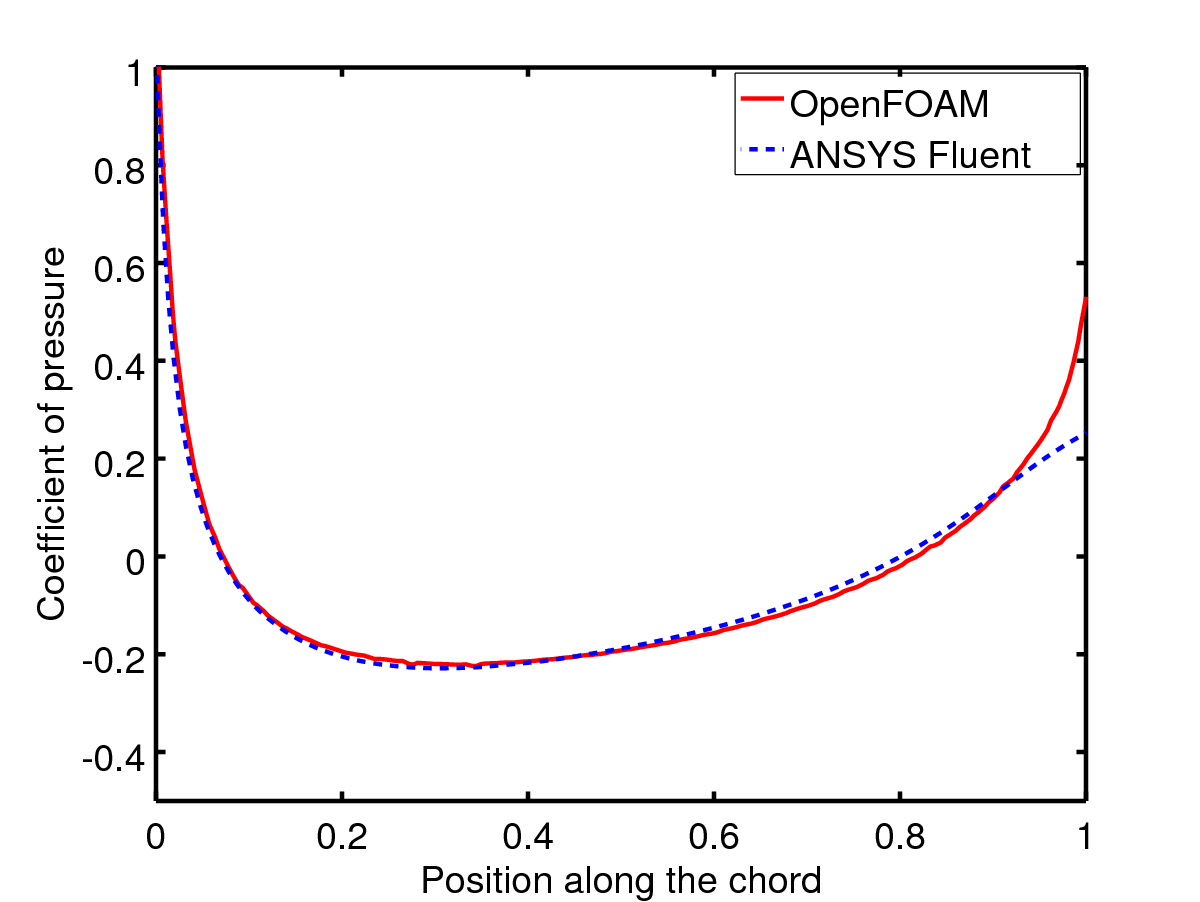
\includegraphics[width=300 pt]{rnd/wang_cp.png}
	\caption{Comparison of OpenFOAM\textsuperscript{\textregistered} results with ANSYS\textsuperscript{\textregistered} \textit{Fluent} results for pressure distribution of Wang shape}
	\label{wang comp} %      only if needed
\end{figure}

Table \ref{wang table} shows the comparison of $ C_{DV} $ obtained using OpenFOAM\textsuperscript{\textregistered} and ANSYS\textsuperscript{\textregistered} \textit{Fluent}

\begin{table}[H]
	\centering
	\caption{\label{wang table} Comparison of OpenFOAM\textsuperscript{\textregistered} results with ANSYS\textsuperscript{\textregistered} \textit{Fluent} for Wang shape}
	%	\begin{ruledtabular}
	\begin{tabular}{cccc}
		\hline \hline
		& OpenFOAM\textsuperscript{\textregistered} & ANSYS\textsuperscript{\textregistered} \textit{Fluent} & \% error \\ \hline \hline
		
		$ C_{DV} $ & 0.02730 & 0.02610 & 4.6    \\ \hline
	\end{tabular}
	%	\end{ruledtabular}
\end{table}


\subsection{NPL Shape \cite{cheeseman2012}}
NPL shaped envelope is basically the combination of two half prolate joint at maximum diameter. It is known for its lower drag characteristics. The mathematical representation of prolate is:
\begin{equation}
\frac{x^{2}}{a^{2}} + \frac{y^{2}}{b^{2}} + \frac{z^{2}}{c^{2}} = 1
\label{NPL_eqn}
\end{equation}
The same surface given by Eq.\ref{NPL_eqn} can also be obtained by rotating the curve given by Eq.\ref{NPL_eqn_2} along X axis
\begin{equation}
y = \begin{cases}
\pm b \sqrt{1-\dfrac{(x-a)^{2}}{a^{2}}} & When \; x \le a \\
\pm b \sqrt{1-\dfrac{(x-a)^{2}}{2a^{2}}} & When \; x \le a
\end{cases}
\label{NPL_eqn_2}
\end{equation}

Values of constants mentioned above are: \textit{a = 82.485  \quad and \quad b = 24.681  }

For the sake of convenience, The surface generated is scaled down by length (\textit{l}) in all directions.The values obtained for finer grid case using OpenFOAM\textsuperscript{\textregistered} are compared with those of using ANSYS\textsuperscript{\textregistered} \textit{Fluent}. 

The flow conditions and solver parameters used for the simulation are shown in Table \ref{Flow conditions and solver parametres for NPL shape}

\begin{table}[H]
	\caption{Flow conditions and solver parametres for NPL shape}
	\label{Flow conditions and solver parametres for NPL shape}
	\centering
	\begin{tabular}{ll}
		\hline \hline
		Flow Conditions & Solver parametres  \\ \hline \hline
		
		$ Velocity = 51 \; m/s$ & $Number \; of \; cells = 1,063,736$    \\  
		$ Pressure = 87500 \; Pa $ & $ Number \; of \; parallel \; cores = 8 $     \\
		$ Density = 1.057 \; kg/m^{3} $ & $ Time \; taken \; for \; solution = 2701 \; s  $    \\
		$ Reynolds \; number = 3.01 * 10^{6} $ &    \\
		$ Turbulence \; model = Spalart \; Allmaras $ &     \\
		\hline
	\end{tabular}
	%	\end{ruledtabular}
\end{table}



Fig. \ref{NPL fig} shows the comparison of $ C_{P} $ distribution using OpenFOAM\textsuperscript{\textregistered} and ANSYS\textsuperscript{\textregistered} \textit{Fluent}
\begin{figure}[H]
	\centering
	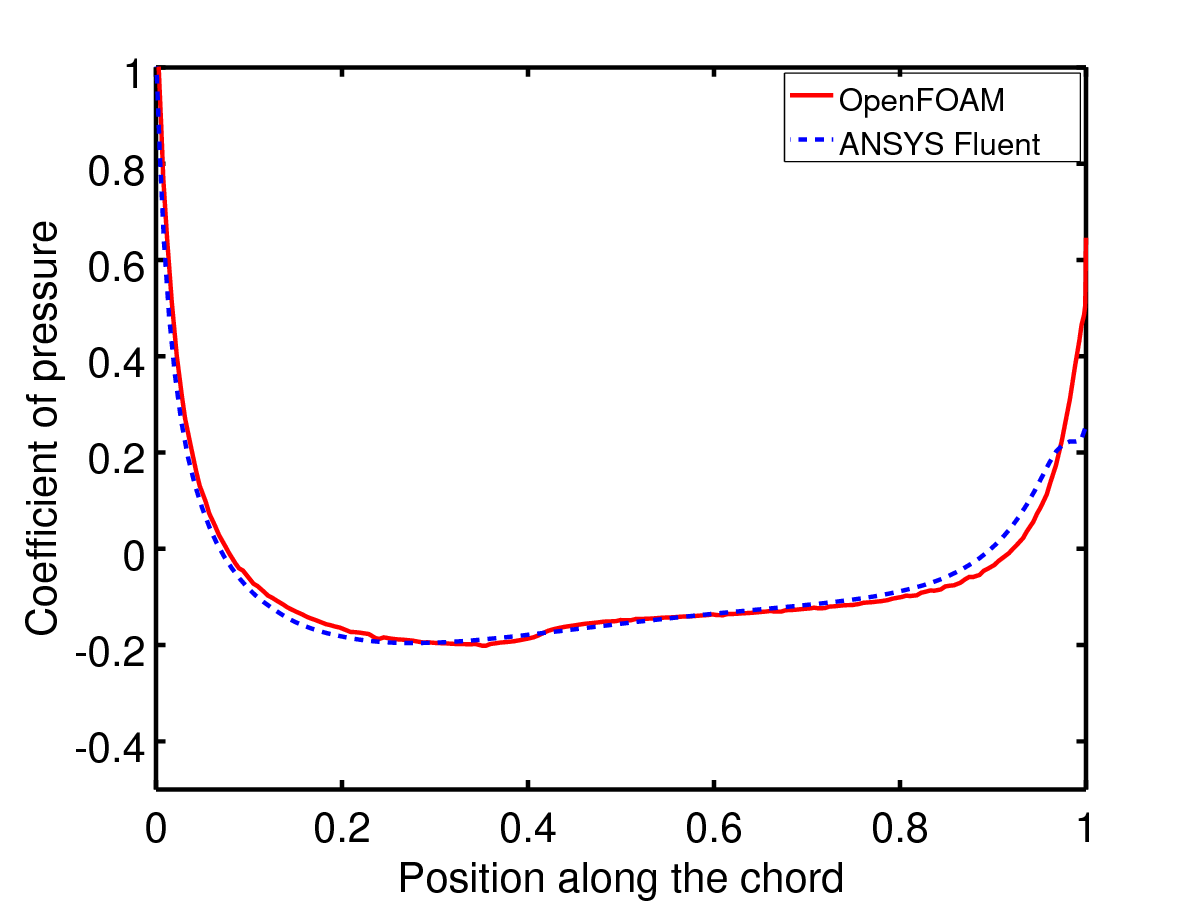
\includegraphics[width=300 pt]{rnd/NPL_cp.png}
	\caption{Comparison of OpenFOAM\textsuperscript{\textregistered} results with ANSYS\textsuperscript{\textregistered} \textit{Fluent} results for pressure distribution of NPL profile \cite{cheeseman2012}}
	\label{NPL fig} %      only if needed
\end{figure} 


Table \ref{NPL table} shows the comparison of $ C_{DV} $ obtained using OpenFOAM\textsuperscript{\textregistered} and ANSYS\textsuperscript{\textregistered} \textit{Fluent}.

\begin{table} [H]
	\centering
	\caption{\label{NPL table} Comparison of OpenFOAM\textsuperscript{\textregistered} results with ANSYS\textsuperscript{\textregistered} \textit{Fluent} for NPL shape}
	%	\begin{ruledtabular}
	\begin{tabular}{cccc}
		\hline \hline
		& OpenFOAM\textsuperscript{\textregistered} & ANSYS\textsuperscript{\textregistered} \textit{Fluent} & \% error \\ \hline \hline
		
		$ C_{DV} $ & 0.02598 & 0.02660 & 2.3    \\   \hline
	\end{tabular}
	%	\end{ruledtabular}
\end{table}

\pagebreak

\subsection{Grid Dependence study}
Since the solution is influenced by mesh size, three self similar grids with increasing number of grid points were considered. Table \ref{GridindependenceGNVR}, \ref{Grid independence study for Wang profile} and \ref{Grid independence study for NPL profile} compares the value for $C_{DV}$ obtained using OpenFOAM\textsuperscript{\textregistered} for GNVR \cite{Ram}, Wang \cite{Wangshape} and NPL\cite{cheeseman2012} shapes respectively.

\begin{table}[H]
	\caption{Grid Dependence study for GNVR shape}
	\label{GridindependenceGNVR} %      only if needed
	\centering
	%	\begin{ruledtabular}
	\begin{tabular}{ c c c c }
		\hline \hline
		& No. of cells & $C_{DV}$ using OpenFOAM\textsuperscript{\textregistered} & \% error change   \\ \hline \hline
		$ Coarse  $ & 198315  & 0.01565 & NA    \\  
		$ Fine $ & 646543  & 0.01555 & 0.6    \\  
		$ Very fine $ & 1444016  & 0.01572 & 1.1    \\ \hline	
	\end{tabular}
	%	\end{ruledtabular}
	
\end{table}

\begin{table}[H]
	\caption{Grid Dependence study for Wang shape}
	\label{Grid independence study for Wang profile} %      only if needed
	\centering
	%	\begin{ruledtabular}
	\begin{tabular}{  c c c c  }
		\hline \hline
		& No. of cells & $C_{DV}$ using OpenFOAM\textsuperscript{\textregistered} & \% error change \\ \hline \hline
		$ Coarse  $ & 1516763 & 0.02709  & NA    \\  
		$ Fine $ & 2494963 & 0.02597  & 10.2    \\  
		$ Very fine $ & 2808841 & 0.02496  & 7.9    \\  \hline	
	\end{tabular}
	%	\end{ruledtabular}
	
\end{table}


\begin{table}[H]
	\caption{Grid Dependence study for NPL shape}
	\label{Grid independence study for NPL profile} %      only if needed
	\centering
	%	\begin{ruledtabular}
	\begin{tabular}{  c  c c c }
		\hline \hline
		& No. of cells & $C_{DV}$ using OpenFOAM\textsuperscript{\textregistered} & \% error change \\ \hline \hline
		$ Coarse  $ & 220813 & 0.02709  & NA    \\  
		$ Fine $ & 1520195 & 0.02597  & 4.1    \\  
		$ Very fine $ & 2521622 & 0.02496  & 3.8    \\  \hline
	\end{tabular}
	%	\end{ruledtabular}
	
\end{table}



According to Suman et al. \cite{suman} if percentage changes compared to previous grid is $\le 5 \%$ then the value obtained from latest grid can be considered as the most accurate. From the above tables we may observe that for GNVR and NPL profiles, the percentage changes are $<$  5 \%, however for Wang profile, they are $>$5 \%. Thus, we can observe that the solution is nearly independent of grid size in all the cases.

\section{Observations \& Conclusions}

From the above results we can observe that OpenFOAM\textsuperscript{\textregistered} results match quite well with those obtained using commercial softwares like ANSYS\textsuperscript{\textregistered} \textit{Fluent} and other proprietary software like RANS \cite{suman}. The likely reasons for the minor differences in the values are as follows:
\begin{itemize}
	\item The results available in literature are 2D simulations using ANSYS\textsuperscript{\textregistered} \textit{Fluent} whereas in our case, they are 3D simulations using OpenFOAM\textsuperscript{\textregistered}.
	\item The mesh is different in the case of ANSYS\textsuperscript{\textregistered} \textit{Fluent} and OpenFOAM\textsuperscript{\textregistered}. OpenFOAM\textsuperscript{\textregistered}'s \textit{SnappyHexMesh} generates the mesh by splitting the cells of structured mesh.
	\item The values of some parameters (e.g., wall functions and wall boundary conditions) had to be assumed because they were not listed in the literature.
\end{itemize}
Apart from the above reasons, OpenFOAM\textsuperscript{\textregistered} solvers are also different from those of ANSYS\textsuperscript{\textregistered} \textit{Fluent}. Only a more detailed and systematic computational study and comparison with reliable experimental data can totally establish the efficacy of OpenFOAM\textsuperscript{\textregistered} w.r.t. ANSYS\textsuperscript{\textregistered} \textit{Fluent} and other proprietary codes.
In last three Chapters, we have discussed about geometry, mesh and solver. Now we have essential tools to carry out shape optimization. The methodology for optimization is discussed in next Chapter.


%%


%%% Local Variables: 
%%% mode: latex
%%% TeX-master: "../mainrep"
%%% End: 

\chapter{Envelope geometry parameterization}
\label{geometry}

Geometry parameterization is an essential part of the design exploration and shape optimization process and there are several methods of generating parametric geometries. Since our ultimate aim of the project is to study different configurations of the non-body-of-revolution shapes and select the best one satisfying our needs. Thus there is a need to parameterize the geometry. Initial attempts were made to parameterize a shape using unconventional methods like polynomial fitting, ruled surface between splines, NURBS (Non Uniform Rational B Splines) etc. The Idea was to define any shape using design variables of not more than 10 because the complexity (time taken, number of function evaluations and memory consumption) of an optimizing problem increases exponentially with number of design variables.

So, the idea was to keep as many less number of design variables as possible provided every combination of them (design variables) gives a meaningful airship shape.

\section{Modified Gertlers parametre technique}

\begin{equation}
\label{eq21}
z^2 = a_1y + a_2y^2 + a_3y^3 + ... + a_ny^n	
\end{equation}
where $a_1$, $a_2$, $a_3$,..., $a_n$ are the shape coefficients, whose values are driven by  geometrical parameters, viz., $m$ (location of maximum diameter), $r_o$ (Nose radius), $r_1$ (tail radius) and $C_p$ (prismatic coefficient), shown in Fig. \ref{fig:cp}. 
\begin{figure}[H]
	\centering
	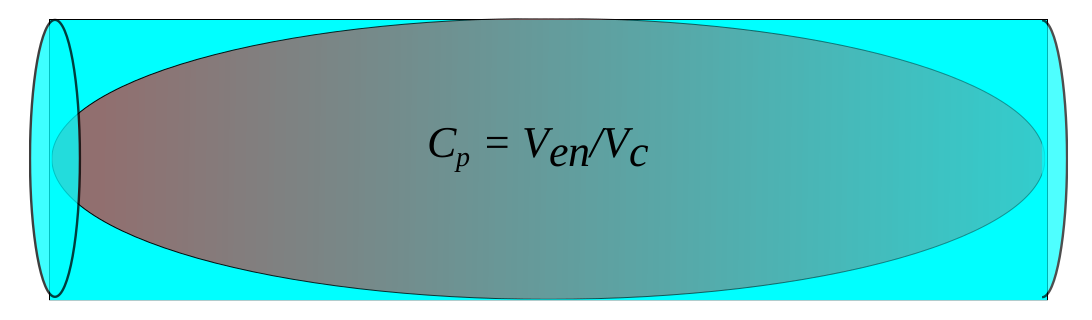
\includegraphics[width=0.7\linewidth]{rnd/c_p_definition.png}
	\caption{Definition of $ Cp $}
	\label{fig:cp}
\end{figure}
By satisfying the various constraints applicable for the shape of a stratospheric airship envelope, the final equations can be obtained in terms of these shape coefficients. To satisfy the constraints applicable for an airship envelope, we apply the conditions $z = 0$, when $y = 1$; $z = 1/2$, when $y = m$ and $\dfrac{dz}{dy} = 0$, when $y = m$, to obtain:
\begin{equation}
a_1 + a_2 + a_3 + ... + a_n = 0	
\end{equation}
\begin{equation}
a_1m + a_2m^2 + a_3m^3 + ... + a_nm^n = \frac{1}{4}	
\end{equation}
\begin{equation}
a_1 + 2a_2m + 3a_3m^2 + ... + na_nm^{n-1} =0	
\end{equation}
Radius of curvature $R$ for any curve can be given as:
\begin{equation}
R = \pm \dfrac{1}{\dfrac{d^2Y}{dZ^2}}\left[1+\left(\dfrac{dY}{dZ}\right)^2\right]^{3/2}
\label{RoC}	
\end{equation}
Eq. \ref {RoC} can be expressed in a  dimensionless form as:
\begin{equation}
\label{eq24}
r = \pm \dfrac{1}{\dfrac{d^2y}{dz^2}}\left[1+\frac{L^2}{D^2}\left(\dfrac{dy}{dz}\right)^2\right]^{3/2}	
\end{equation}
Differentiating Eq. \ref{eq21} successively with respect to y we get:
\begin{equation}
\label{eq22}
2z = \left(a_1 + 2a_2y +...+ na_n^{n-1}\right)\dfrac{dy}{dz}
\end{equation}
and
\begin{equation}
\label{eq23}
2 = \left(a_1 + 2a_2y +...+ na_n^{n-1}\right)\dfrac{d^2y}{dz^2} + \left[2a_2 + ...+n(n-1)a_n^{n-2}\right]\left(\dfrac{dy}{dz}\right)^2
\end{equation}
In Eq. \ref{eq22}, if $a_1\ne 0$ then it can be said that when $x = 0$, $\dfrac{dy}{dz} = 0$, and hence from the Eq. \ref{eq23}, that
$\dfrac{d^2y}{dz^2} = \dfrac{2}{a_1}$. Consequently substituting these values in Eq. \ref{eq24} we can get:
\begin{equation}
\label{eq25}
a_1 = 2r_o
\end{equation}
where $r_o$ is the radius of curvature at the nose. If, on the other hand $a_1 = 0$, then $r_o = 0$, i.e., the body has pointed nose, which is not possible for an inflated envelope. Hence, Eq. \ref{eq25} is valid for both the cases.\\
Similarly, when $y = 1$, $z = 0$ and from Eq. \ref{eq22},     $\dfrac{dy}{dz} = 0$, unless:
\begin{equation}
\label{eq26}
a_1 + 2a_2 + 3a_3 +...+na_n = 0
\end{equation}
Hence, Eq. \ref{eq24} and Eq. \ref{eq23} give:
\begin{equation}
\label{eq27}
a_1 + 2a_2 + 3a_3 +...+na_n = -2r_1
\end{equation}
where $r_1$ is the radius of curvature at the tail. Different signs are taken in equation of $r_o$ and $r_1$ because of the nature of slope at the points $y = 0$ and $y = 1$ respectively.

Volume of the envelope ($ V_{env}) $ can be expressed as:
\begin{equation}
V_{env} = \int_{0}^{l}\pi Z^2 dY = \pi d^2L\int_{0}^{1}z^2dy	
\end{equation}
substituting for $z^2$ from Eq. \ref{eq21} we get,
\begin{equation}
\dfrac{1}{2}a_1	+ \dfrac{1}{3}a_2 + \dfrac{1}{4}a_3+ ... + \dfrac{1}{n+1}a_n = \dfrac{1}{4}C_p
\end{equation}

The aforementioned six constraints can be expressed in the form of a six degree polynomial as follows:
\begin{equation}
z^2(0) = 0
\end{equation}
\begin{equation}
z^2(1) \implies a_1 + 2a_2 + 3a_3 +...+na_n = 0
\end{equation}
\begin{equation}
\dfrac{dz}{dy}\Big|_0 \implies a_1= 2r_o
\end{equation}
\begin{equation}
\dfrac{dz}{dy}\Big|_1 \implies a_1 + 2a_2 + 2a_3 +...+na_n = -2r_1
\end{equation}
\begin{equation}
z^2(m)\implies a_1m + a_2m^2 + a_3m^3 + ... + a_nm^n = \frac{1}{4}	
\end{equation}
\begin{equation}
\dfrac{dz}{dy}\Big|_m \implies a_1 + 2a_2m + 3a_3m^2 + ... + na_nm^{n-1} =0	
\end{equation}
\begin{equation}
\int_{0}^{1} z^2(y)dy \implies \dfrac{1}{2}a_1	+ \dfrac{1}{3}a_2 + \dfrac{1}{4}a_3+ ... + \dfrac{1}{n+1}a_n = \dfrac{1}{4}C_p
\end{equation}

The above-mentioned linear equations can be represented in a Matrix form as:
\begin{equation}
A\bm{Y} = B
\end{equation}
\[
\begin{bmatrix}
1 & 1 & 1 & 1 & 1 & 1 \\
1 & 0 & 0 & 0 & 0 & 0 \\
1 & 2 & 3 & 4 & 5 & 6 \\
m & m^2 & m^3 & m^4 & m^5 & m^6 \\
1 & 2m & 3m^2 & 4m^3 & 5m^4 & 6m^5 \\
\dfrac{1}{2} & \dfrac{1}{3} & \dfrac{1}{4} & \dfrac{1}{5} & \dfrac{1}{6} & \dfrac{1}{7} \\
\end{bmatrix}
\\
\begin{bmatrix}
a_1\\
a_2\\
a_3\\
a_4\\
a_5\\
a_6\\
\end{bmatrix}
=
\begin{bmatrix}
0\\
2r_o\\
-2r_1\\
\dfrac{1}{4}\\
0\\
\dfrac{1}{4}C_p\\
\end{bmatrix}
\]


There are six unknowns in these six linear equations, hence $\bm{Y}$ can be obtained for a set of geometrical parameters by solving these equations simultaneously. The final equation for airship envelope shape can be rewritten as:
\begin{equation}
\label{eq28}
z(y) = D\sqrt{a_1\left(\dfrac{y}{L}\right) + a_2\left(\dfrac{y}{L}\right)^2 + a_3\left(\dfrac{y}{L}\right)^3 + a_4\left(\dfrac{y}{L}\right)^4 + a_5\left(\dfrac{y}{L}\right)^5 +  a_6\left(\dfrac{y}{L}\right)^6}	
\end{equation}
The obtained curve is then rotated about X-axis to get axisymmetric shape. However to get a non axisymmetric shape, we introduce a new variable called $ scale_y $ which when multiplied with the y-coordinates of the body changes it into non-axisymmetric shape. The below figure shows the effect of scaling.
\begin{figure}[htbp]
	\centering
	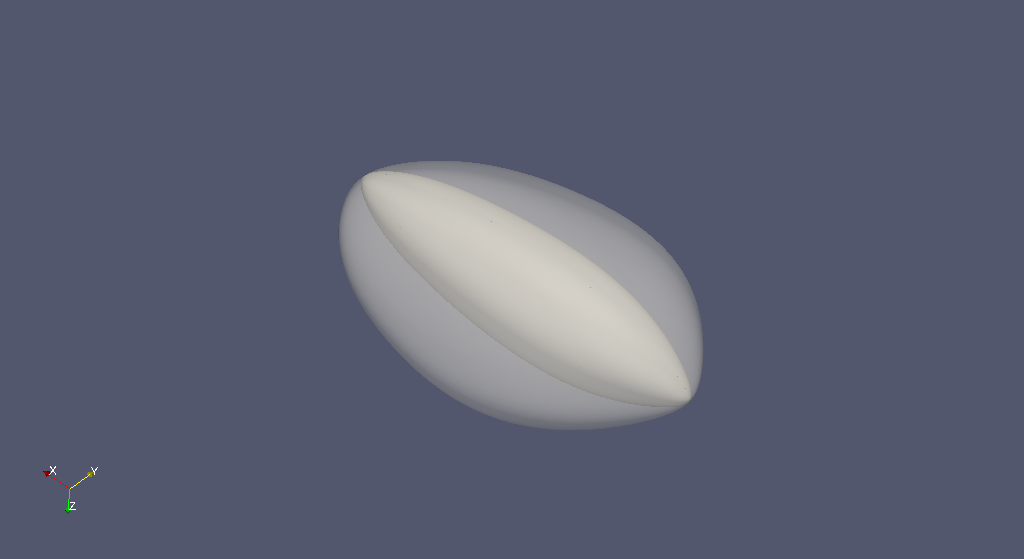
\includegraphics[width=200 pt]{rnd/effect_of_scaling.png}
	\caption{Effect of scaling }
	\label{Effect of scaling}
\end{figure}


\section{Methodology to generate surface using \textit{Octave}}

Since the analysis work is being carried out using OpenFOAM\textsuperscript{\textregistered}, we need to input the geometry file to \textit{SnappyHexMesh} utility. OpenFOAM\textsuperscript{\textregistered} don't have any geometry creation utility. We need to create the geometry using any commercial designing software and export the file to .stl format and carryout the analysis. During optimization, Calling the commercial CAD software every time to define simple mathematical shape is not a good practise. Instead we can define the geometry in Octave itself and carryout simulations. So, an existing MATLAB\textsuperscript{\textregistered} script has been edited which takes the input of surface data  (X,Y and Z vectors) and writes them into .stl file. This .stl file can then be used in OpenFOAM\textsuperscript{\textregistered}. So, the need for commercial designing software has been eliminated positively.
\subsection{STL (file format)}
An ASCII STL file begins with the line
\begin{lstlisting}
solid name
\end{lstlisting}



where name is an optional string (though if name is omitted there must still be a space after solid). The file continues with any number of triangles, each represented as follows:
\begin{lstlisting}
facet normal ni nj nk 
	 outer loop	
		vertex v1x v1y v1z 
		vertex v2x v2y v2z 
		vertex v3x v3y v3z 
	 endloop 
endfacet 
\end{lstlisting}

where each n or v is a floating-point number in sign-mantissa-"e"-sign-exponent format, e.g., "2.648000e-002". The file concludes with the line,


\begin{lstlisting}
endsolid name
\end{lstlisting}

Thus the \textit{surf} data consisting of x,y,z coordinates of all the points are written into a text file in the above format and can be imported into OpenFOAM\textsuperscript{\textregistered} to carryout CFD simulation.

Next chapter discusses why OpenFOAM\textsuperscript{\textregistered} has been used for CFD analysis when we have industry standard commercial CFD softwares.

%%


%%% Local Variables: 
%%% mode: latex
%%% TeX-master: "../mainrep"
%%% End: 

\chapter{Surrogate based shape optimization}
\label{optimization}
The usual way of doing any CFD geometry optimization is shown in ~\ref{Closed Optimization loop}. But following this procedure is not feasible because it takes a lots of computational effort and time. Also, grid influences the solution considerably. So, using this method we can no longer guarantee that the changes in the solution of objective function value is because of the changes in the parameters of CAD or if they are coming from changes in the grid. The solution for the problems can be answered by developing a surrogate model.
\begin{figure}[H]
	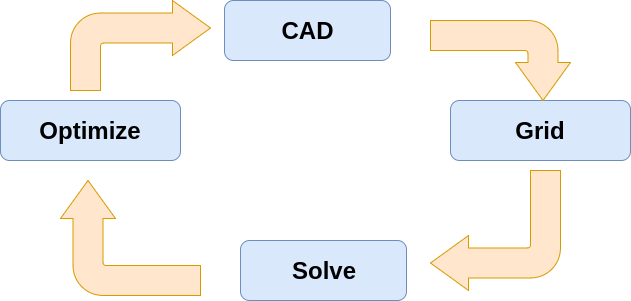
\includegraphics[width=\textwidth]{optimization/closed_loop.png}
	\caption{Closed Optimization loop}
	\label{Closed Optimization loop} %      only if needed
\end{figure}

\section{Surrogate model}

 Surrogate model is one of the mathematical and statistical techniques used to develop adequate functional relationship between an objective function y(x) and the control or design variables $ x_1 , x_2 .... x_k $. In our case, The model acts like a black box for aerodynamic parameters. Given the set of design variables, the model should give volumetric drag coefficient as shown in Figure \ref{Surrogate model} . The work flow associated with the development of a surrogate model is shown in Figure ~\ref{fig:work flow for the development of a surrogate model} . To develop an accurate surrogate, we need to carry out large number of CFD simulations. Creating geometry every time and meshing them is possible but takes a lot of time. Instead we can automate all the processes right from geometry creation to meshing and solving. This has become possible with OpenFOAM\textsuperscript{\textregistered}.

\begin{figure}[H]
	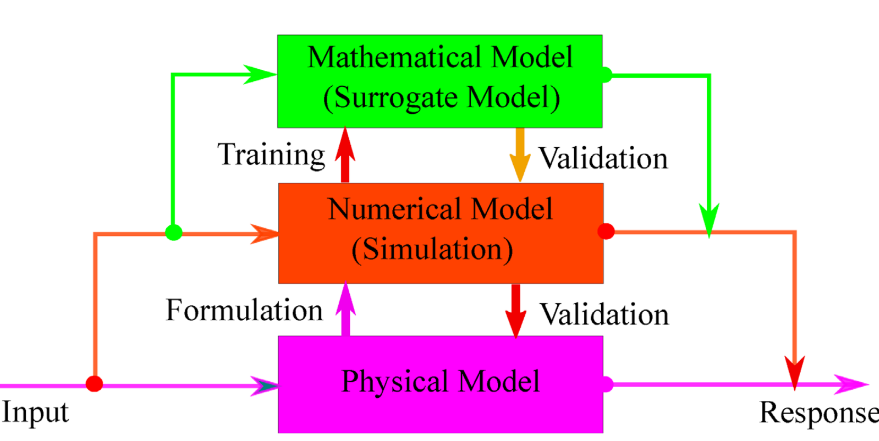
\includegraphics[width=\textwidth]{optimization/surrogate.png}
	\caption{Surrogate model definition}
	\label{Surrogate model} %      only if needed
\end{figure}

%\begin{figure}[htbp]
%	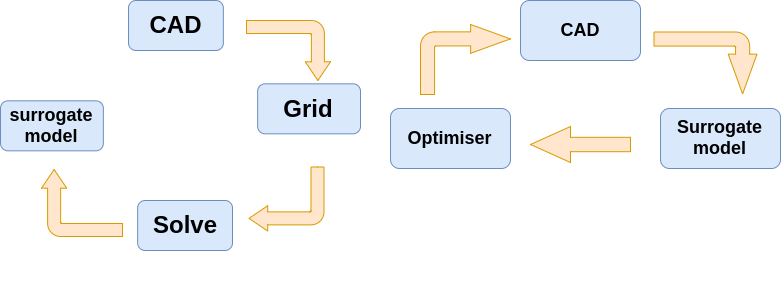
\includegraphics[width=\textwidth]{optimization/model.png}
%	\caption{Broken Optimization loop with the use of surrogate model}
%	\label{Broken Optimization loop with the use of surrogate model} %      only if needed 
%\end{figure}

\begin{figure}[htbp]
	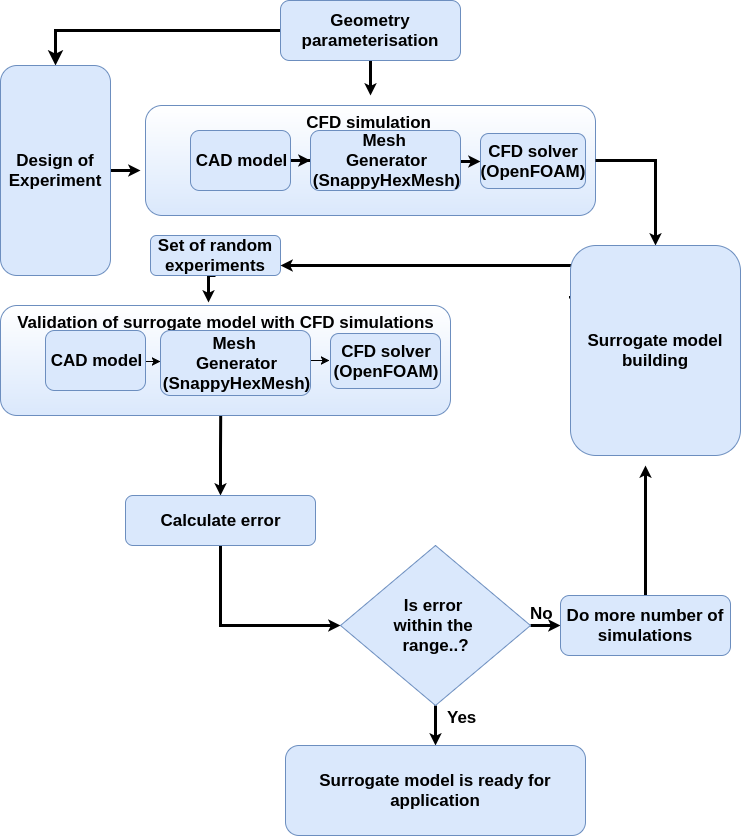
\includegraphics[width=\textwidth]{optimization/flow_chart.png}
  
	\caption{work flow for the development of a surrogate model}
	\label{fig:work flow for the development of a surrogate model} %      only if needed
\end{figure}


\section{Design of Experiments}
\label{DOE}
Design of Experiments is a technique used to extract maximum possible information from minimum number of computational experiments. This can be accomplished by the selection of a proper and robust scheme for DOE (Design of Experiments). In the present study, an open-source software named Surrogates Toolbox Version 3.0 (Viana, 2011) was used. Apart from many other important features, the toolbox provides an access to several varieties of widely used DOE models. Of the many DOE models available in the toolbox, optimal Latin Hypercube Sampling (OLHS) generated using translational propagation algorithm (TPA) \textbf{cite Viana et. al} was chosen, mainly due to its orthogonal structure. Fig. \ref{OLHS Sampling} shows sampling distribution of points in a unit square.

\begin{figure}[htbp]
	\centering
	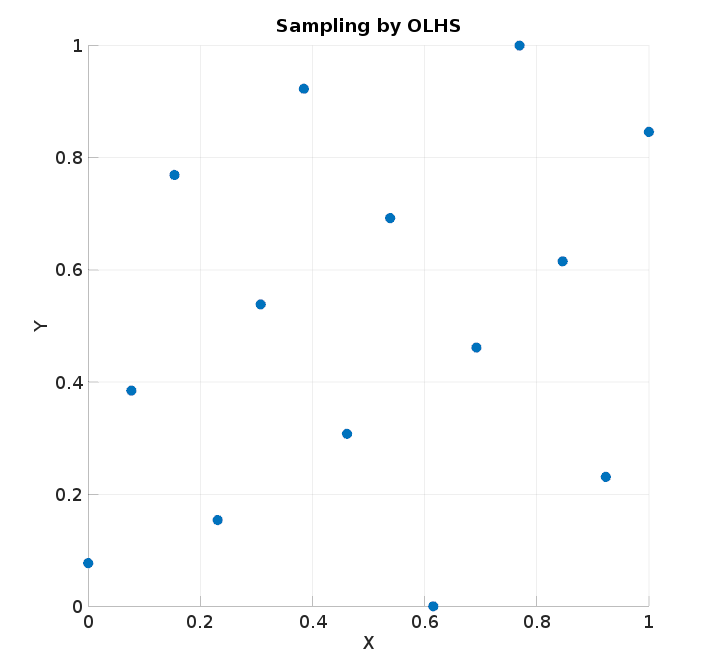
\includegraphics[width=200 pt]{optimization/OLHS_DOE}
	\caption{Sampling of unit square using OLHS }
	\label{OLHS Sampling}
\end{figure}

 The number of design experiments depends on the number of shape parameters used for defining geometry. A rule of thumb is that the number of design experiments should be ten times the number of shape parametres. However the actual number is decided by obtaining error between surrogate model results and actual CFD results. For the surrogate model to be acceptable, the error should be less than 2 percent. \cite{alam2016mdo} reported to have made 80 design experiments while developing his surrogate model for 2D bodies of revolution shapes. \cite{Kale2005a} reported to have studied about 600 feasible shapes using ANSYS\textsuperscript{\textregistered} \textit{Fluent} CFD package while developing quadratic response surface using Design Expert package.

For numerical experiments, Kriging surrogate model is reported to be best \citenum{viana2014metamodeling}. Kriging is named after the pioneering work of the South African mining engineer D. G. Krige. It is an interpolating method modelled by a Gaussian process governed by prior co-variances, which features the observed data at all design points. Kriging provides a statistic prediction of an unknown function by minimizing its Mean Squared Error (MSE).

The Kriging method in its basic formulation estimates the value of a function at some un sampled location as the sum of two components: the linear regression model $ f_i (x) $ (e.g., polynomial trend) of the data with p regressors modelling the drift of the process mean, i.e., the trend, over the domain, and a systematic departure representing low (large scale) and high frequency (small scale) variation components, respectively.


\section{Test Function for Kriging Surrogate Model}
The Himmelblau function is taken as a test function.  It has one local maxima and four local minima in the domain x = [-6,6] and y = [-6,6]. The function is defined as 
\begin{equation}
f(x,y) = (x^2 + y - 11)^2  + (x + y^2 - 7)^2 
\end{equation}
\begin{equation}
x \in [-6,6] ;\quad y \in [-6,6]
\end{equation}

It has one local maximum at x=-0.270845 and y=-0.923039 where f(x,y)=181.617, and four identical local minima:
\begin{align}
&f( 3.0000 , 2.0000 )=0.0 \\
&f( -2.8051 , 3.1313 )=0.0 \\
&f( -3.7793 , -3.2831 )=0.0 \\
&f( 3.5844 , -1.8481 )=0.0 \\
\end{align}

If a small number of design points are used to create a surrogate model, then the approximate model created is prone to large errors at the trial points. However, the prediction accuracy of a surrogate model cannot be improved merely by taking larger number of design points; that is a function of its behaviour, design space and the required accuracy. Fig. \ref{fig:Root Mean Square Error with Design Points considered} shows the effect of increase in number of design points on the Root Mean Square Error (RMSE) of this test function. It is seen that the prediction accuracy of the model improves till 120 design points, after which addition of more design points does not approximate model for surrogate on the right with all the design points and test points. The actual value fo the function and predicted value from the surrogate model at test points are seen to match with each other within 1\%.

\begin{figure}[H]
	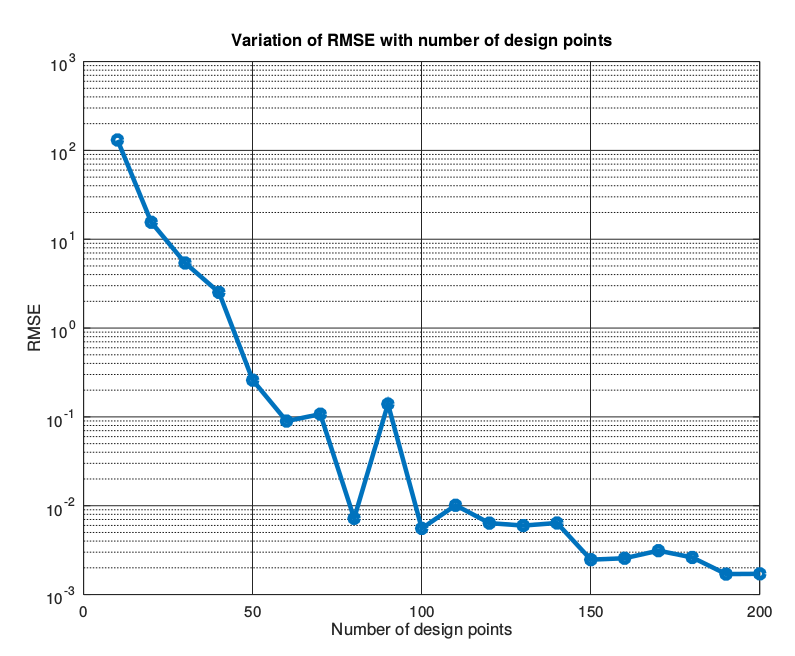
\includegraphics[width=\textwidth]{optimization/RMSE_analysis.png}
	\caption{Root Mean Square Error with Design Points considered}
	\label{fig:Root Mean Square Error with Design Points considered} %      only if needed
\end{figure}


\begin{figure}[H]
	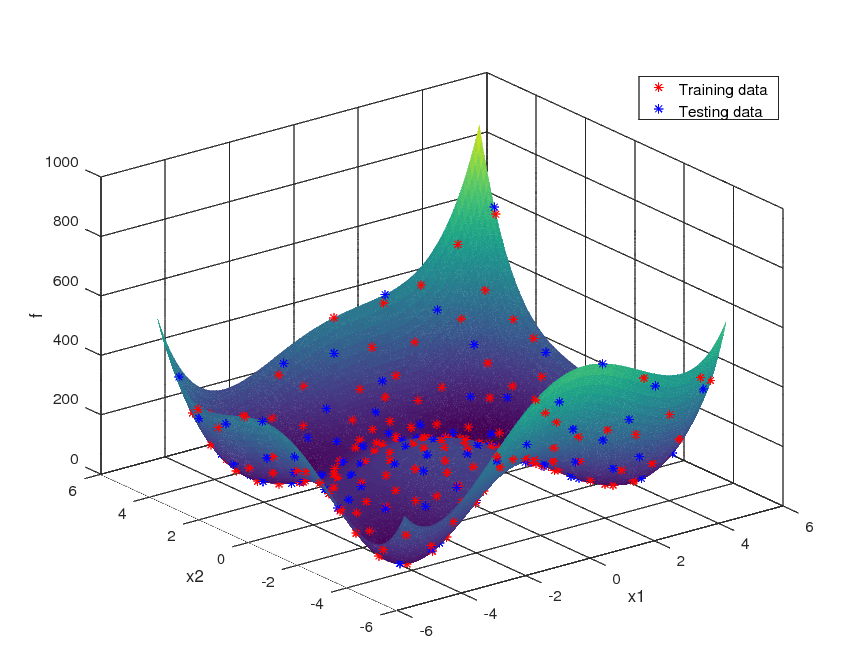
\includegraphics[width=\textwidth]{optimization/Himmel_blau_fcn.png}
	\caption{Comparison of Himmelblau function with its Surrogate Model}
	\label{fig:Comparison of Himmelblau function with its Surrogate Model} %      only if needed
\end{figure}

\section{Coupling of Genetic Algorithm, Surrogate model and testing for modified Himmelblau functions}
It is a well known fact that evolutionary algorithms like Genetic algorithm searches for global minimum and outputs that global minimum as final answer. Unlike gradient based methods, it should not get struck in local minimum. In order to check this, we modify the existing Himmelblau function. This is because actual Himmelblau function has four identical local minimum and don't have any global mimima. So, we modify it by adding the term $  0.01* (x + 3.7793)^2 + (y + 3.2832)^2 $. This term is added to the function value evaluated at all points except (-3.7793,-3.2832). Hence we obtained modified Himmelblau function with one global minima at (-3.7793,-3.2832) and three local minima at other three points. If we optimise this modified Himmelblau function using Genetic algorithm, we have to get the final answer as (-3.7793,-3.2832). The same answer is expected using surrogate model for the modified Himmelblau function. The obtained results are shown in Table.

\begin{table}[H]
	\centering
	\caption{Results obtained for modified Himmelblau function}
	\label{Results obtained for modified Himmelblau function}
	%\begin{ruledtabular}
	\begin{tabular}{llll}
		\hline \hline
		& X & Y & Function value \\ \hline
		Actual Function & -3.7793 &-3.2832 &1.6725e-11 \\
		Surrogate model & -3.7791 &-3.2828 & 2.5643e-03 \\ \hline
		\% error & 0.006 & 0.013 & 2.5643e-03 \\
		\hline \hline
		
		
		
		
	\end{tabular}
	%	\end{ruledtabular}
\end{table}






%%


%%% Local Variables: 
%%% mode: latex
%%% TeX-master: "../mainrep"
%%% End: 

\chapter{Surrogate model for CFD}
To develop a surrogate model which mimics the behaviour of CFD in finding the drag coefficient at zero degree angle of attack, it is essential to identify the limits of design parameters, perform Design Of Experiments (DOE) on them, perform CFD analysis at these DOE points and fit a surrogate model. The whole processes is described in the subsections below.

\section{Mapping design variables}
The first task before creation of DOE was the proper definition of the upper and lower limits for the six design variables (viz., $ m, r_0, r_1, C_p, \frac{l}{d} \ and \  scale \_y $). The upper and lower limits of design variables are calculated using the initial sizing done by \cite{alam2017thesis}. The design space is confined as mentioned in Table \ref{Degign space }

\begin{table}[H]
	\centering
	\caption{Design Space}
	\label{Degign space }
	%\begin{ruledtabular}
	\begin{tabular}{lll}
		\hline \hline
		Design Parameters & Min. & Max.    \\ \hline \hline
		
		$ Point\ of\ Max.\ Dia., m$ & 0.35 & 0.50     \\  
		$ Nose\ Radius, r _{o} $ & 0.20 & 0.80     \\
		$ Tail\ Radius, r _{1} $ & 0.1 & 0.5     \\  
		$ Prismatic\ Coeff., C _{p }$ & 0.55 & 0.70 \\
		$ Fineness\ Ratio, \frac{l}{d} $ &2.50 & 6.00 \\
		$Scaling\ in\ Y\ direction,\ scale\_y$ &1.00 & 5.00\\ \hline \hline
	\end{tabular}
	%	\end{ruledtabular}
\end{table}

Eighty candidate points were first obtained by Surrogates Toolbox \textbf{cite surrogate toolbox} using the Optimal Latin Hypercube Sampling (OLHS) method. The generated points were then mapped to the shapes corresponding to envelope volume ($ V _{env} $ ) of 250000 $ m^3 $ . 

\section{Design of Experiments study}

As mentioned previously in section \ref{DOE}, DOE study is used to extract maximum amount of information from every experiment conducted. This is especially needed when we are carrying out expensive computer or real life experiments. While developing surrogate model for CFD, each CFD analysis will take about 3 hours to complete. Hence to optimally use the computation resources, the total number experiments needs to be as low as possible but extracting maximum information about function behaviour. So, initially the number of experiments are taken as 80 and the design points are generated using the Optimal Latin Hypercube Sampling (OLHS) technique present in SURROGATES Toolbox by \cite{viana2014metamodeling}. The obtained points are given in Appendix.

\section{CFD analysis on the points obtained from DOE}

All the pre-processing required to perform CFD analysis like creating the geometry, deciding the size of domain, meshing the domain has been automated using Octave and C++ scripting. The scripts are shared in Appendix.
\section{Building the surrogate model}
A brief overview of different surogate models by \cite{luo2014comparison} is given below.
\subsection{Polynomial response surface}
Polynomial response surface is the simplest approximation method to build surrogate models \cite{forrester2009recent}. The most widely used polynomial response surface model is the second-order polynomial model which has the following form.
\begin{equation}
y = \beta _{0} + \sum_{i=1}^{n} \beta _{i} x_{i} + \sum_{i=1}^{n} \sum_{j \ge i}^{n} \beta _{ij} x_{i} x_{j} + ..
\end{equation}

where $ \beta _{0},\ \beta_{i},\ \beta _{ii},$ and $ \beta _{ij} $ are the regression coefficients, n is the number of variables, xi and xj are the variables. Using least square method (LSM), the regression coefficients can be solved.

\subsection{Radial basis function}
RBF is a 3-layer feed forward neural network consisting of an input layer, a hidden layer, and an output layer \cite{shen2011forecasting}. X is an N dimensional input vector. The output of the neurons in the RBF hidden layer is assumed as:

\begin{equation}
q_{i} = \varPhi(|| X - c_{i} ||)
\end{equation}

where $ c_{i} $ is the center associated with the ith neuron in the radial basis function hidden layer, i = 1, 2,...,H, where H is the number of hidden units, $ || X - c_{i} || $ is the norm of $ X − c_{i} $, $ \varPhi (.) $ is a radial basis function \cite{chen1991orthogonal}. Outputs of the kth neuron in RBF output layer are linear combinations of the hidden layer neuron outputs as:

\begin{equation}
	y_{k} = \sum_{i=1}^{H} w_{ki} q_{i} - \theta _{k} \quad (k = 1, 2,...,M)
\end{equation}
where $ w_{ki} $ is the connecting weights from the $ i^{th} $ hidden layer neuron to the $ k^{th} $ output layer, $ \theta _{k} $ is the threshold value of the $ k^{th} $ output layer neuron.

\subsection{Kriging}
The kriging method was developed by the French mathematician Georges Matheron based on the Master$ ' $s thesis of Daniel Gerhardus Krige \cite{matheron1963principles}, it was first used as a geostatistical method. \cite{sacks1989design} firstly introduced kriging method as a surrogate modelling method, in the paper of \cite{sacks1989design}, kriging surrogate model was also called design and analysis of computer experiment (DACE). The kriging model is a combination of two components \cite{queipo2005surrogate}: deterministic functions and localized deviations.

\begin{equation}
Y(x) = \sum_{i=1}^{k} f_{i} (x) \beta _{i} + z(x)
\end{equation}

where $ \sum_{i=1}^{k} f_{i} (x) \beta _{i} $ is the term of deterministic functions, $ \beta$ are coefficients of deterministic functions, fi(x) are k known regression functions, which are usually polynomial functions. z(x) is term of localized deviations with mean zero, variance σ2, and covariance expressed as:

\begin{equation}
Cov[z(x_{i}),z(x_{j})] = \sigma ^{2} R (x_{i},x_{j})
\end{equation}

where $ R (x_{i},x_{j}) $  is the correlation function between any two of the ns samples The common types of correlation functions are linear function, exponential function, Gauss function, spline function, etc. (Ryu et al. 2002). 
The prediction of unsampled points response y(x) can be expressed as:

\begin{equation}
\hat{y}(x) = f(x)^{T} \beta + r^{T} R^{-1} (Y - F \beta )
\end{equation}

where Y is the vector of ns samples response, r is the correlation vector between samples and prediction points.


\begin{eqnarray}
& r = [R(x,x_{1}),R(x,x_{1}),....,R(x,x_{1}) ]^{T} \\
& F = [f(x_{1}), f(x_{2}),.....f(x_{n_{x}}) ]^{T} .
\end{eqnarray}

\section{Toolbox used for different surrogate models}

Table \ref{Different surrogates used during this investigation} details the different surrogates used during this investigation. The SURROGATES toolbox was also used for easy manipulation of the surrogates.

Table \ref{Different surrogates used during this investigation}: Setup for the set of used surrogates. The  DACE \citenum{lophaven2002dace}, RBF \citenum{Jekabsons2009} and SURROGATES \citenum{Viana2011} toolboxes were used to run the kriging, radial basis function and polynomial response surface respectively.

\begin{table}[H]
	\centering
	\caption{Different surrogates used during this investigation}
	\label{Different surrogates used during this investigation}
	%\begin{ruledtabular}
	\begin{tabular}{ll}
		\hline \hline
		Surrogate & Details    \\ \hline \hline
		 KRG	 & Kriging model: constant trend function and Gaussian correlation \\
		 PRS & Polynomial response surface: Second degree polynomial \\
		 RBF  & Radial basis function: Multiquadric basis function \\
		 \hline \hline
	\end{tabular}
	%	\end{ruledtabular}
\end{table}







\chapter{Training data of CFD results to train surrogate model}
In our case, 80 DOEs are generated and steady state 3D CFD analysis has been performed for these 80 shapes. The solver parameters used are as follows:
\begin{table}[H]
	\caption{Flow conditions and solver parametres for all DOE shapes}
	\label{Flow conditions and solver parametres for all DOE shapes}
	\centering
	\begin{tabular}{ll}
		\hline \hline
		Parameters & Value \\ 
		\hline \hline
		Reynolds number based on volume Re & $ 3.01 \ast 10^6 $ \\
		Pressure, N/m2 & 87500 \\
		Density, Kg/m3 & 1.057 \\
		Speed, m/s & 51 \\
		Mesh & Hexahedral mesh using blockMesh and snappyHexMesh \\
		Solver & SimpleFOAM (Incompressible steady state solver) \\
		Turbulent..? & Yes \\
		Turbulence model & K-Omega SST \\
		\hline \hline
	\end{tabular}
\end{table}
\section{Grid Convergence study}

Effect of grid size on the overall results by  changing the number of cells in self similar mesh has been carried out. Below is the plot of variation of pressure and viscous drag with number of cells for a simulation. As mentioned by \cite{Suman2011} , when the percentage change in the values is less than 5 \%, then the solution is reported to have grid convergence.

\begin{table}[H]
	\caption{Grid convergence study}
	\label{Grid convergence table}
	\centering
	\begin{tabular}{ccc}
		\hline \hline
		Cells & Pressure Drag (N) & Viscous Drag (N) \\
		\hline \hline
		376380 & 1.1  & 11.02 \\
		604375  & 2.2  & 11.68 \\
		840565  & 2.02  & 12.1 \\
		994864  & 2.09  & 12.24 \\
		1563471  & 2.12 & 12.5 \\
		\hline \hline
	\end{tabular}
\end{table}

\begin{figure}[H]
	\centering
	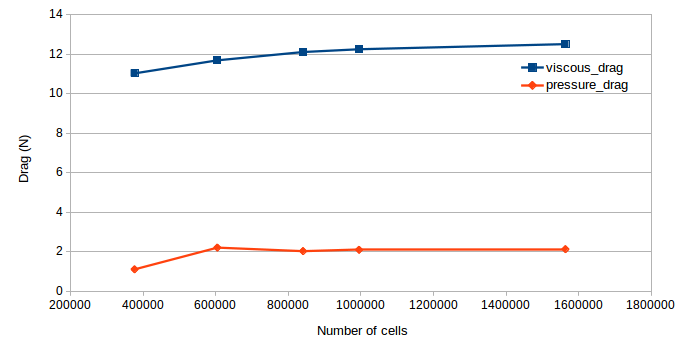
\includegraphics[width=300 pt]{surrogate_model_CFD_results/Grid_convergence.png}
	\caption{Variation of pressure and viscous drag with number of cells}
	\label{Grid convergence plot} %      only if needed
\end{figure}



\chapter{Calculation of Hoop Stress}
\label{Hoop stress}

In order to maintain positive pressure inside the envelope, three main loadings are considered to estimate the internal over pressure ($ \Delta P $) viz., the loading due to dynamic pressure, aerodynamic loading, and hydro-static pressure as suggested by Gupta \& Malik \cite{gupta2002envelope} . A brief description of these three components of the module is as given below.

\textbf{Dynamic Pressure}: Dynamic pressure loading acts on the front portion of the aerostat envelope and tries to make a depression on the envelope surface, its diameter depends on the region of highly stressed area which is normally 7 to 9 \% of the envelope length. To maintain the shape of the envelope, the internal pressure is kept slightly higher than dynamic pressure, normally 15\% as suggested by Gupta \& Malik \cite{gupta2002envelope} as per Eq. \ref{dyn}
\begin{equation}
\label{dyn}
\Delta P_{dyn} = 1.15 \bigg( \frac{1}{2} \rho_{air} v^{2} \bigg)
\end{equation}

\textbf{Aerodynamic Pressure}: Aerodynamic pressure loading results from applying the stability conditions to the airship. Coefficient of pressure, as observed normally for airship profiles is in the range of 0.30 to 0.35 from the leading edge, but normally for such shapes, it is assumed at the maximum diameter. is used for calculating the pressure due to this loading.

\begin{equation}
\label{aer}
\Delta P_{aer} = c_{p} \bigg( \frac{1}{2} \rho_{air} v^{2} \bigg)
\end{equation}

\textbf{Hydrostatic Pressure}: Hydrostatic pressure loading is due to the difference between the height of the top and bottom of aerostat and could be quite substantial of the aerostat diameter in large. The hydrostatic pressure as observed at mean centerline axis of the envelope is calculated at maximum diameter using:

\begin{equation}
\label{hyd}
\Delta P_{hyd} = \frac{1}{2} (\rho _{air} - \rho_{He} ) g D_{c}
\end{equation}
The sum of pressure due to these three loadings gives the total required internal pressure. Since the aerostat envelope diameter is more than twenty times of the thickness of the material; it can be considered as a very thin shell and hence hoop stress is calculated in terms of the circumferential unit load as shown in Eq. \ref{sum_delta}
\begin{equation}
\label{sum_delta}
\Delta P = \Delta P_{dyn} + \Delta P_{aer} + \Delta P_{hyd}
\end{equation}
To estimate the longitudinal stress ($ \sigma _{l} $ ) and the circumferential hoop stress ($ \sigma _{h} $) developed in an envelope, an equivalent cylindrical envelope is considered, having the same surface area and volume as the actual airship envelope, as shown in Fig \ref{Stress representation in envelope}

\begin{figure}[H]
	\centering
	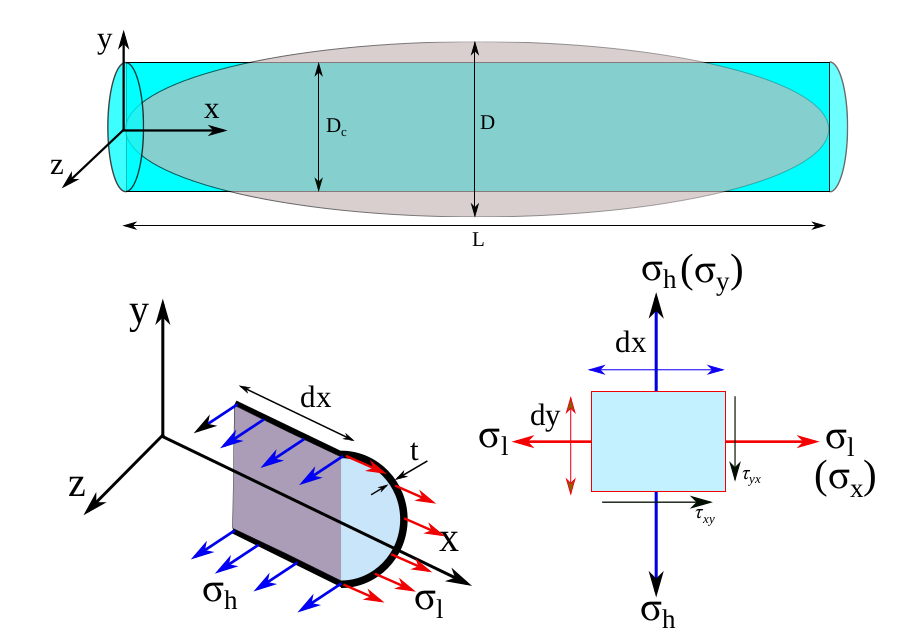
\includegraphics[width=0.7\linewidth]{von_mises/stress_rep_envelope.png}
	\caption{Stress representation in envelope}
	\label{Stress representation in envelope}
\end{figure}
Hence, $ \sigma _{l} $ and $ \sigma _{h} $ developed in an envelope are estimated as:

\begin{equation}
 \sigma _{h} = \frac{\Delta P D_{c}}{2}
\end{equation}

\begin{equation}
\sigma _{l} = \frac{\Delta P D_{c}}{4}
\end{equation}

To maintain the aerodynamic shape and rigidity of an airship envelope some pressure difference ( $ \Delta P^{'} $ ) is also needed, which can be determined by bending moment estimation.

\subsection{Bending Moment Calculation}

An empirical relation for maximum bending moment given by FAA \citenum{cheeseman1999} can be expressed as:
\begin{equation}
\label{moment_eqn}
M = 0.029 [1 + (f-4)(0.5624L^{0.02} - 0.5)]\ \rho _{air} . u . v . V_{env} L^{0.25}
\end{equation}
Where D, is the diameter of airship envelope with the where u and v are the gust and wind velocity respectively. Eq. \ref{moment_eqn} is valid for fineness ration between 4 to 6. For fineness ratio less than 4, f can be assumed as 4.
The point at which the maximum bending moment occurs, i.e., near the center of gravity, $ \sigma _{l} $ at the top of this must be greater than or equal to zero. Therefore, the equation for $ \sigma _{l} $ can be written as:

\begin{equation}
\label{eqn_for_sima_l}
\sigma _{l} = \dfrac{ \Delta P^{'} \pi R^{2} } {2 \pi R } - \frac{MRT}{I} \ge 0
\end{equation}

Where R is the radius of airship envelope at the point of maximum bending. \textit{t} is the thickness the envelope material. \textit{I} is the second moment of area, which has the value of $ \pi R^{3} t $. Minimum pressure required $ \Delta P^{'} $ to maintain the shape of the envelope can be calculated as:

\begin{equation}
\Delta P^{'} = \frac{16M}{\pi D^{3} }
\end{equation}

Where D is the diameter of airship envelope with the assumption that, the location of maximum bending is same as the location of maximum diameter. Total differential pressure ∆P t can be obtained as:
\begin{equation}
\Delta P_{t} = max(\Delta P , \Delta P ^{'})
\end{equation}
In that case, $ \sigma _{h} $ and  $ \sigma _{l} $ can be calculated as:

\begin{equation}
\sigma _{h} = \frac{\Delta P D_{c}}{2}
\end{equation}
\begin{equation}
\sigma _{l} = \frac{\Delta P D}{4} + \frac{4M}{\pi D^{2} }
\end{equation}

\textbf{von-Mises Stress Calculation}: From the principle stresses, von-Mises stress can be expressed as:

\begin{equation}
\sigma _{v} = \Bigg[ \frac{(\sigma _{1}  - \sigma _{2})^2 + (\sigma _{2}  - \sigma _{3})^2 + (\sigma _{3}  - \sigma _{1})^2 }{2}   \Bigg]^{\frac{1}{2}}
\end{equation}

Stresses are considered only in 2-D planes due to very low thickness of envelope compared to its diameter. Therefore $ \sigma _{3} $ = 0, which simplifies the equation as:

\begin{equation}
\sigma _{v} = \sqrt{\frac{(\sigma _{1} - \sigma _{2})^{2} + \sigma _{1} ^{2} + \sigma _{2} ^{2}}{2}}
\end{equation}

\begin{equation}
\sigma _{v} = \sqrt{\sigma _{1} ^{2} + \sigma _{2} ^{2} - \sigma _{1} \sigma _{2}}
\end{equation}

\section{Shape for minimum hoop stress}
An octave function namely $ Von_Mises.m $ has been written incorporating the concepts of section \ref{Hoop stress}. This function gives the value of von-Mises stress ($ \sigma _{v} $) given the values of design parametres shown in Table \ref{Degign space }. The optimal results obtained are as follows:
\begin{table}[H]
	\centering
	\caption{Optimal solution obtained for miminum $ \sigma _{v} $}
	\label{Optimal solution obtained for mimimum sigma_v}
	%\begin{ruledtabular}
	\begin{tabular}{lc}
		\hline \hline
		Design Parameters & Optimal value for minimum $ C_{DV} $    \\ \hline \hline
		
		$ Point\ of\ Max.\ Dia., m$ & 0.44960      \\  
		$ Nose\ Radius, r _{o} $ & 0.38316    \\
		$ Tail\ Radius, r _{1} $ & 0.23247     \\  
		$ Prismatic\ Coeff., C _{p }$ & 0.60598 \\
		$ Fineness\ Ratio, \frac{l}{d} $ &4.28392 \\
		$Scaling\ in\ Y\ direction,\ scale\_y$ &1.50423 \\ \hline \hline
		
		$ von-Mises\ stress\  \sigma _{v}  $ & \\
		\hline \hline
	\end{tabular}
	%	\end{ruledtabular}
\end{table}

%%% Local Variables: 
%%% mode: latex
%%% TeX-master: "../mainrep"
%%% End: 

\chapter{Work done in Stage-1}
\label{results}





%%% Local Variables: 
%%% mode: latex
%%% TeX-master: "../mainrep"
%%% End: 

\chapter{Future work}
\label{future plan}


\appendix
\chapter{Table of design points obtained from OLHS}

%****************************************************************
%                         Appendices                           
%****************************************************************
%% Additional, supporting material, such as codes, derivations, etc., can be placed in the appendix


%******************************************************************
%                         Bibliography or References          
%******************************************************************  
\bibliography{mylit.bib}     

%*******************************************************************
%                         List of publications               
%******************************************************************
%%%%
\listofpublications


\noindent Put your publications from the thesis here. The packages \texttt{multibib} or \texttt{bibtopic} or \texttt{biblatex} or enumerate environment or thebibliography environment etc. can be used to handle multiple different bibliographies in the document.








%%======================================================================
%%% Local Variables: 
%%% mode: latex
%%% TeX-master: "../mainrep"
%%% End: 







            

%*******************************************************************
%                        Acknowledgements                    
%******************************************************************* 
%%%%
\acknowledgments

This section is for the acknowledgments. Please keep this brief and resist the temptation of writing flowery prose! Do include all those who helped you, e.g. other faculty/staff you consulted, colleagues who assisted etc.






\signature{\today}
%\signature[Indian Institute of Technology Bombay]{\today}

%========================================================================

%%% Local Variables: 
%%% mode: latex
%%% TeX-master: "../mainrep"
%%% End:            

%*******************************************************************
%                        About author                    
%*******************************************************************
%\colophon % remove this command while using this file.

% GAME OVER
%*******************************************************************
\end{document}

%%% Local Variables: 
%%% mode: latex
%%% TeX-master: t
%%% End: 
